
\documentclass[%
 reprint,
%superscriptaddress,
%groupedaddress,
%unsortedaddress,
%runinaddress,
%frontmatterverbose, 
%preprint,
%preprintnumbers,
nofootinbib,
%nobibnotes,
%bibnotes,
 amsmath,amssymb,
 aps,
%pra,
%prb,
%rmp,
%prstab,
%prstper,
floatfix,
]{revtex4-2}
\usepackage{gensymb}
\usepackage{textcomp}
\usepackage{lipsum}
\usepackage{graphicx}% Include figure files
\usepackage{dcolumn}% Align table columns on decimal point 


\usepackage{bm}% bold math
\usepackage{siunitx}
\DeclareSIUnit\gauss{G}
\DeclareSIUnit\erg{erg}
\DeclareMathOperator{\Rot}{rot}
\sisetup{separate-uncertainty=true}
\usepackage{tabularx}
\usepackage{amssymb}
\usepackage{amsmath}
\usepackage{relsize}
\usepackage{commath}
\usepackage{enumitem}
\usepackage{xfrac}
\usepackage{float}
\usepackage{booktabs}
\usepackage{makecell}
\usepackage{caption}
\usepackage{subcaption}
\usepackage{multirow}
\usepackage[version=4]{mhchem}
\usepackage[colorlinks,bookmarks=false,citecolor=blue,linkcolor=blue,urlcolor=blue]{hyperref}
%\usepackage{hyperref}% add hypertext capabilities
%\usepackage[mathlines]{lineno}% Enable numbering of text and display math
%\linenumbers\relax % Commence numbering lines

%\usepackage[showframe,%Uncomment any one of the following lines to test 
%%scale=0.7, marginratio={1:1, 2:3}, ignoreall,% default settings
%%text={7in,10in},centering,
%%margin=1.5in,
%%total={6.5in,8.75in}, top=1.2in, left=0.9in, includefoot,
%%height=10in,a5paper,hmargin={3cm,0.8in},
%]{geometry}

\begin{document}

\preprint{APS/123-QED}

\title{Experiments with Geiger-M\"{u}ller Counter}% Force line breaks with \\


\author{Maitrey Sharma}
\email{maitrey.sharma@niser.ac.in}
\affiliation{School of Physical Sciences, National Institute of Science Education and Research, HBNI, Jatni-752050, India}




\date{\today}% It is always \today, today,
             %  but any date may be explicitly specified

\begin{abstract}
    In this experiment, we perform various experiments using the Geiger-M\"{u}ller Counter and understand the working of the electronics and physics behind it. We first examine the characteristic curve of the G-M tube and study the terminology involved there. Then we move on to the gamma radiation and how its intensity depends with distance. Then we indulge ourselves in the statistical analysis of the data obtained through a G-M counter experiment as we study the randomness of radioactive decay. Afterwards, we study the efficiency of our G-M counter and how it varies with gamma or beta source. Then we perform the Feather analysis due to Norman Feather, who contributed to the discovery of neutron with Chadwick. We then move on to study the phenomena of backscattering of the beta particles. After this, we encounter the phenomena of Bremsstrahlung and how it is produced. Finally we measure the short half-life of a given radioactive source.
\end{abstract}

\keywords{Bohr’s atomic model, quantisation of energy levels, electron spin, Bohr’s magneton, interference of electromagnetic waves, Fabry-Perot interferometer}
\maketitle

%\tableofcontents

\section{\label{sec:level1}Introduction}
    In 1908 Hans Geiger, under the supervision of Ernest Rutherford at the Victoria University of Manchester (now the University of Manchester), developed an experimental technique for detecting alpha particles. This early counter was only capable of detecting alpha particles and was part of a larger experimental apparatus and used a fundamental ionization mechanism used discovered by John Sealy Townsend between 1897 and 1901, known as the Townsend discharge\footnote{The Townsend discharge or Townsend avalanche is a gas ionisation process where free electrons are accelerated by an electric field, collide with gas molecules, and consequently free additional electrons. Those electrons are in turn accelerated and free additional electrons. The result is an avalanche multiplication that permits electrical conduction through the gas.}. It was not until 1928 when Geiger and his student Walther M\"{u}ller developed a sealed tube which used basic ionization principles previously used experimentally. Small and rugged, not only could it detect alpha and beta radiation as prior models had done, but also gamma radiation, giving birth to a practical radiation instrument which could be produced relatively cheaply. As the tube output required little electronic processing, a distinct advantage in the thermionic valve era due to minimal valve count and low power consumption, the instrument achieved great popularity as a portable radiation detector.
    \begin{figure}
        \centering
        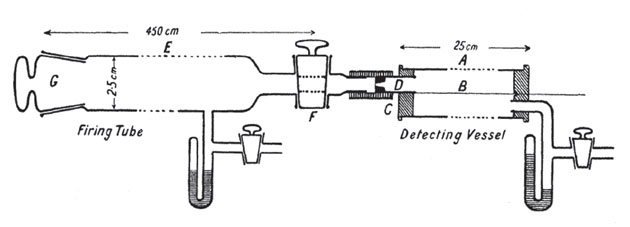
\includegraphics[scale = 0.35]{Figures/PSM_V87_D120_Apparatus_for_counting_alpha_particles.png}
        \caption{An early alpha particle counter designed by Rutherford and Geiger.}
        \label{fig:ruthercount}
    \end{figure}
    \par
    A Geiger–M\"{u}ller (G-M) counter is an electronic instrument used for detecting and measuring ionizing radiation. It detects ionizing radiation such as alpha particles, beta particles, and gamma rays using the ionization effect produced in a Geiger–M\"{u}ller (G-M) tube, which gives its name to the instrument.
    \par
    The G-M tube is named after Hans Geiger, who invented the principle in 1908 at the University of Manchester, and Walther M\"{u}ller, who collaborated with Geiger in developing the technique further in 1928 to produce a practical tube that could detect a number of different radiation types. It is a gaseous ionization detector and uses the Townsend avalanche phenomenon to produce an easily detectable electronic pulse from as little as a single ionizing event due to a radiation particle. It is used for the detection of gamma radiation, X-rays, and alpha and beta particles. It can also be adapted to detect neutrons.
    \par
    A G-M Tube consists of basically an electrode at a positive potential (anode) surrounded by a metal cylinder at a negative potential (cathode). The cathode forms part of the envelope or is enclosed in a glass envelope. Ionizing events are initiated by quanta or particles, entering the
    tube either through the window or through the cathode and colliding with the gas molecules. The gas filling consists of a mixture of one or more rare gases and a quenching agent. Quenching is the termination of the ionization current pulse in G-M tube. Effective quenching in G-M Tube is determined by the combination of the quenching gas properties and the value of the anode resistor.
    \begin{figure}
        \centering
        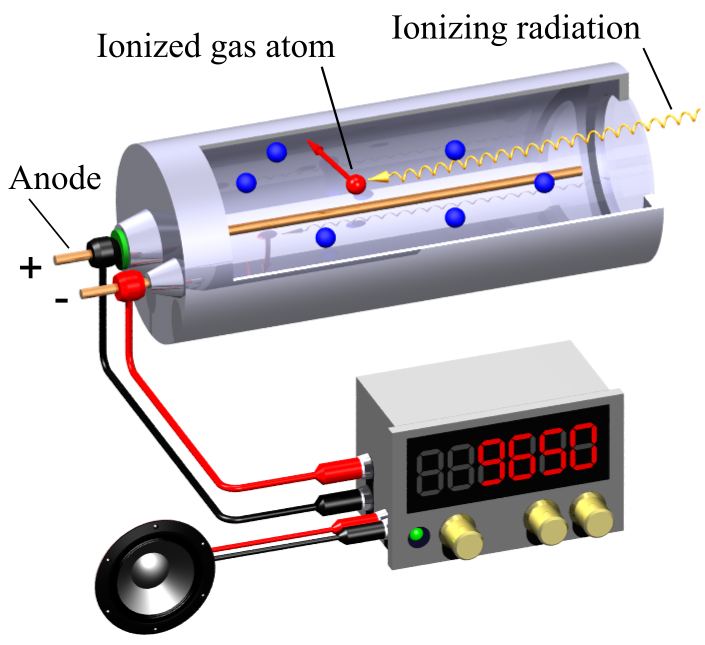
\includegraphics[scale = 0.4]{Figures/Geiger-Muller-counter-en.png}
        \caption{Diagram of a Geiger counter using an end window tube for low penetration radiation. A loudspeaker is also used for indication}
        \label{fig:maingm}
    \end{figure}

\section{Description of the Set-up}
    In this experiment, we will be using the cylindrical ``end window'' type pf G-M tube construction (figure (\ref{fig:maingm})), which is the usual form of tube for alpha particles, low energy beta particles, and low energy X-rays. This type has a window at one end covered in a thin material through which low-penetrating radiation can easily pass. Mica is a commonly used material due to its low mass per unit area. The other end houses the electrical connection to the anode. The complete experimental apparatus is presented in figure (\ref{fig:expt-setup}).
    \begin{figure}
        \centering
        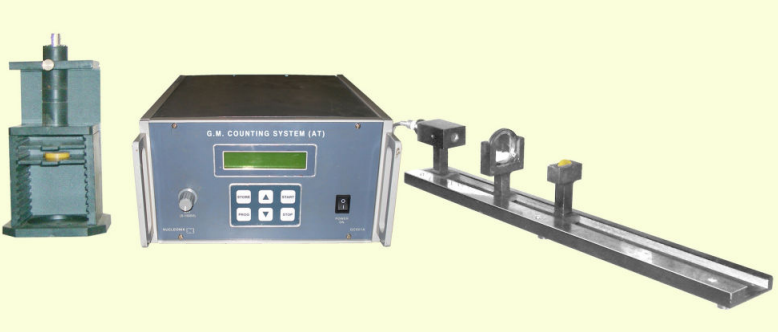
\includegraphics[scale = 0.45]{Figures/gmcounting.png}
        \caption{G-M counting system with End window detector stand and sliding bench}
        \label{fig:expt-setup}
    \end{figure}
    The experimental set-up of the counting experiments has several components, each of which are described in this section.
    \begin{enumerate}
        \item \textbf{\textit{Geiger counting system:}} The main counting system device designed around a 8-bit microcontroller chip. 
        \item \textbf{\textit{Detector:}} \textit{GM 120} is a Halogen Quenched End Window G-M Detector used in the experiment.  Its operating voltage is approximately $\SI{500}{\volt}$. It has got a very wide plateau length and plateau slope is better than 6\% per $\SI{100}{\volt}$. This detector is supplied in a cylindrical PVC enclosure with MHV (miniature high voltage) socket arrangement for applying HV (high voltage) bias voltage.
        \item \textbf{\textit{Stand for the detector:}} Stand for G-M tube type \textit{SG 200} has been designed to hold PVC enclosed End Window G-M tube. This standcan be housed inside the lead shielding if required. It has both   sample and absorber trays. The position of these trays can be  adjusted from the end window of the detector. The stand made up  of acrylic sheet is precisely milled for sliding-in of sample and absorber trays. Sample tray is designed to hold planchets or disc  type radioactive standard source (Beta or Gamma). Aluminium absorber discs can be interposed between the source and the detector for attenuating the radiation as seen by the detector.
        \par
        Captive screw holds the detector PVC tube to any height. To increase the distance between end window and source one can lift the PVC tube further up which can be held by captive screw. The detector apparatus is presented in figure (\ref{fig:stand}).
        \begin{figure}
            \centering
            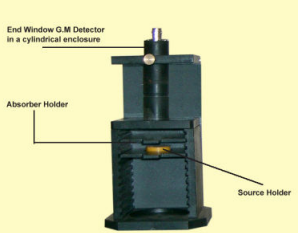
\includegraphics[scale = 0.9]{Figures/detector stand.png}
            \caption{G-M detector stand}
            \label{fig:stand}
        \end{figure}
        \item \textbf{\textit{Sliding Bench:}} This essentially consists of a bench with sliding groves with a graduated stainless steel scale fixed on one side of it. Scale has graduations both in cm and inches upto 50cm/20 inches. There are three vertical sliding mounts, each for mounting of End Window G-M detector horizontally facing the absorber and source mounts. Each of these mounts can be positioned along the slide scale to have required distance between the end window to the source with absorber mount interposed in between. End Window detector is housed in PVC enclosure with MHV socket fixed on to it. The sliding bench apparatus is presented in figure (\ref{fig:slidingbench}).
        \begin{figure}
            \centering
            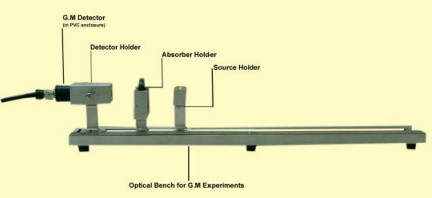
\includegraphics[scale = 0.85]{Figures/slidingbench.png}
            \caption{Sliding bench for the G-M experiments}
            \label{fig:slidingbench}
        \end{figure}
        \item \textbf{\textit{Source kits:}} These kits contain the radioactive (Beta and Gamma) sources. These are low active disc sources of the order of 0.2 to 3 micro curie for Beta and Gamma. Gamma source disc is evaporated and sealed inside 25mm (diameter) $\times$ 5mm thick plastic disc. Whereas Beta source disc is evaporated and sealed in a 25mm $\times$ 10mm thick plastic disc and covered with 10mg/ sq.cm aluminised mylar foil.
        \item \textbf{\textit{Aluminium absorber set:}} It consists of absorber discs in different thicknesses ranging from 20 to 300 mg/cm.sq. Each of these absorbers is mounted in an individual plastic frame, which exactly fits into the absorber tray holder of the detector stand/sliding bench.
        \item \textbf{\textit{Lead castle:}} The Lead Castle is designed to shield the G-M Counters from counting background radiation. This shield is of 40 mm thickness and is built up of six interlocking rings. The top and bottom are covered by similar interlocking discs. A door is fitted in the bottom ring with 150 degree opening to facilitate easy access to the sample holding tray of G-M Stand. The door is fitted with heavy duty hinges and the inside of the lead shield is lined with thin aluminium sheet to minimize scattering.
        \item \textbf{\textit{Absorber/scatterer sets:}} The absorber/scatterer set used in the Beta-particle scattering experiment consists of 15 Aluminium foils, the thickness of each foil being 0.05 mm. The one used in the Bremsstrahlung experiment consists of combinations of Aluminium (0.7 mm thick), along with Copper (0.3 mm thick) and Perspex (1.8 mm thick).
    \end{enumerate}

    
    
\section{The Experiments}
    Before beginning the experiments, it is essential to calculate the present activity rates of the radioactive sources. We know, the activity is given by
    \begin{equation}
    \label{eq:act}
        A = A_0 e^{- \lambda t} = A_0 e^{-(0.693/T_{1/2})t}
    \end{equation}
    where $A$ is the present activity, $A_0$ is the activity on a previous date $T_{1/2}$ is the half-life of the source, $t$ is the elapsed time and $\lambda$ is the decay constant.
    \begin{itemize}
        \item \textbf{Thallium-204} \textit{(Beta source)}: We have $A_0 = \SI{11}{\kilo \becquerel}$ (in May 2016), $T_{1/2} = 4$ years, $t = 5.67$ years (by February 2022), putting these values in equation (\ref{eq:act}), we get $A = \SI{4120.34}{\becquerel}$.
        \item \textbf{Strontium-90} \textit{(Beta source)}: We have $A_0 = \SI{3.7}{\kilo \becquerel}$ (in May 2019), $T_{1/2} = 28.5$ years, $t = 2.67$ years (by February 2022), putting these values in equation (\ref{eq:act}), we get $A = \SI{3467.65}{\becquerel}$.
        \item \textbf{Caesium-137} \textit{(Gamma source)}: We have $A_0 = \SI{86}{\kilo \becquerel}$ (in May 2016), $T_{1/2} = 30$ years, $t = 5.67$ years (by February 2022), putting these values in equation (\ref{eq:act}), we get $A = \SI{75446.18}{\becquerel}$.
    \end{itemize}
    
    \subsection{Characteristics of Geiger-M\"{u}ller Tube}
    \label{sec:GMtubecharac}
        The first experiment is concerned with the characteristics of the G-M counter. We will study the variations of count-rate with applied voltage and thereby determine the plateau, the operating voltage and the slope of the plateau. The equipment used are the G-M counting system, the end window detector stand, the G-M detector itself and a radioactive source.
        \begin{figure}
            \centering
            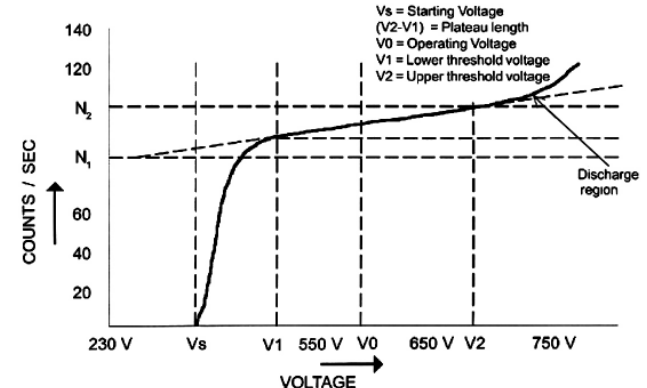
\includegraphics[scale = 0.63]{Figures/typicalgmcharac.png}
            \caption{Typical G-M characteristics}
            \label{fig:typicalGM}
        \end{figure}
        \begin{figure}
            \centering
            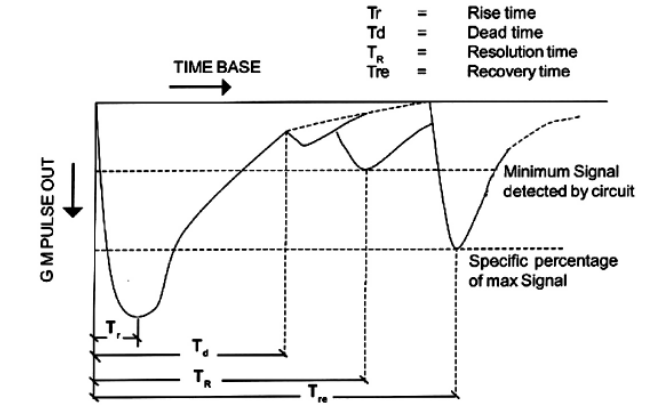
\includegraphics[scale = 0.63]{Figures/gmpulseout.png}
            \caption{Typical G-M pulse output as seen on an oscilloscope}
            \label{fig:gmpulseout}
        \end{figure}
        \par
        There are various operating characteristics of the G-M tube which define how it behaves when irradiated constantly. The lowest voltage applied to a G-M tube at which pulses just appear across the anode resistor (figure (\ref{fig:typicalGM})) and unit starts counting is called the \textbf{\textit{starting voltage}}, $V_s$. The section of the G-M characteristic curve constructed with counting rate versus applied voltage (with constant irradiation) over which the counting rate is substantially independent of the applied voltage is called the \textbf{\textit{plateau}} and the voltage range over which it extends is called the \textbf{\textit{plateau length}}. The slope of the plateau line is referred as the \textbf{\textit{plateau slope}}. The two voltages, corresponding to the start and the end of the plateau are called the \textbf{\textit{lower}} ($V_1$) and \textbf{\textit{upper threshold voltages}} ($V_2$) respectively. The average of these two is taken as the \textbf{\textit{operating voltage}}, $V_0$ of the G-M tube.
        
        The radioactive source used is the Cs-137 gamma source. The observations made are tabulated in table (\ref{tab:GMcharac}). The background counts represent the counts in absence of the source, due to cosmic rays or any other sources in the location of experiment.
            
        \newcommand{\ra}[1]{\renewcommand{\arraystretch}{#1}}
        \begin{table*}[]
        \ra{1.3}
        \caption{Readings for the G-M characteristics experiment}
        \label{tab:GMcharac}
        \setlength{\tabcolsep}{12pt}
        \begin{tabular}{@{}ccccccccccccccccccc@{}}
        \toprule
        \begin{tabular}[c]{@{}c@{}}\textbf{EHT} \\ (V)\end{tabular} & \phantom{abc} &
          \multicolumn{3}{c}{\begin{tabular}[c]{@{}c@{}}\textbf{Background} \\ \textbf{counts}\\ (30 s)\end{tabular}} & \phantom{abc} &
          \multicolumn{3}{c}{\begin{tabular}[c]{@{}c@{}}\textbf{Counts}\\ (30 s)\end{tabular}} & \phantom{abc} &
          \multicolumn{3}{c}{\begin{tabular}[c]{@{}c@{}}\textbf{Corrected} \\ \textbf{Counts}\\ (30 s)\end{tabular}} \\ \midrule
        330 && 0  & 0  & 0  && 0    & 0    & 0    && 0    & 0    & 0    \\
        360 && 14 & 36 & 35 && 3432 & 3282 & 3270 && 3418 & 3246 & 3235 \\
        390 && 27 & 26 & 32 && 3780 & 3834 & 3817 && 3753 & 3808 & 3785 \\
        420 && 32 & 25 & 23 && 3971 & 3876 & 3823 && 3939 & 3851 & 3800 \\
        450 && 33 & 33 & 43 && 3861 & 3931 & 4015 && 3828 & 3898 & 3972 \\
        480 && 44 & 28 & 33 && 4013 & 3972 & 3954 && 3969 & 3944 & 3921 \\
        510 && 23 & 27 & 27 && 4091 & 4099 & 3866 && 4068 & 4072 & 3839 \\
        540 && 31 & 25 & 40 && 4098 & 4078 & 3996 && 4067 & 4053 & 3956 \\
        570 && 40 & 30 & 22 && 4037 & 4193 & 4168 && 3997 & 4163 & 4146 \\
        600 && 30 & 29 & 23 && 4267 & 4113 & 4104 && 4237 & 4084 & 4081 \\
        630 && 66 & 56 & 46 && 7633 & 7781 & 7694 && 7567 & 7725 & 7648 \\ \bottomrule
        \end{tabular}
        \end{table*}
        \begin{figure}
            \centering
            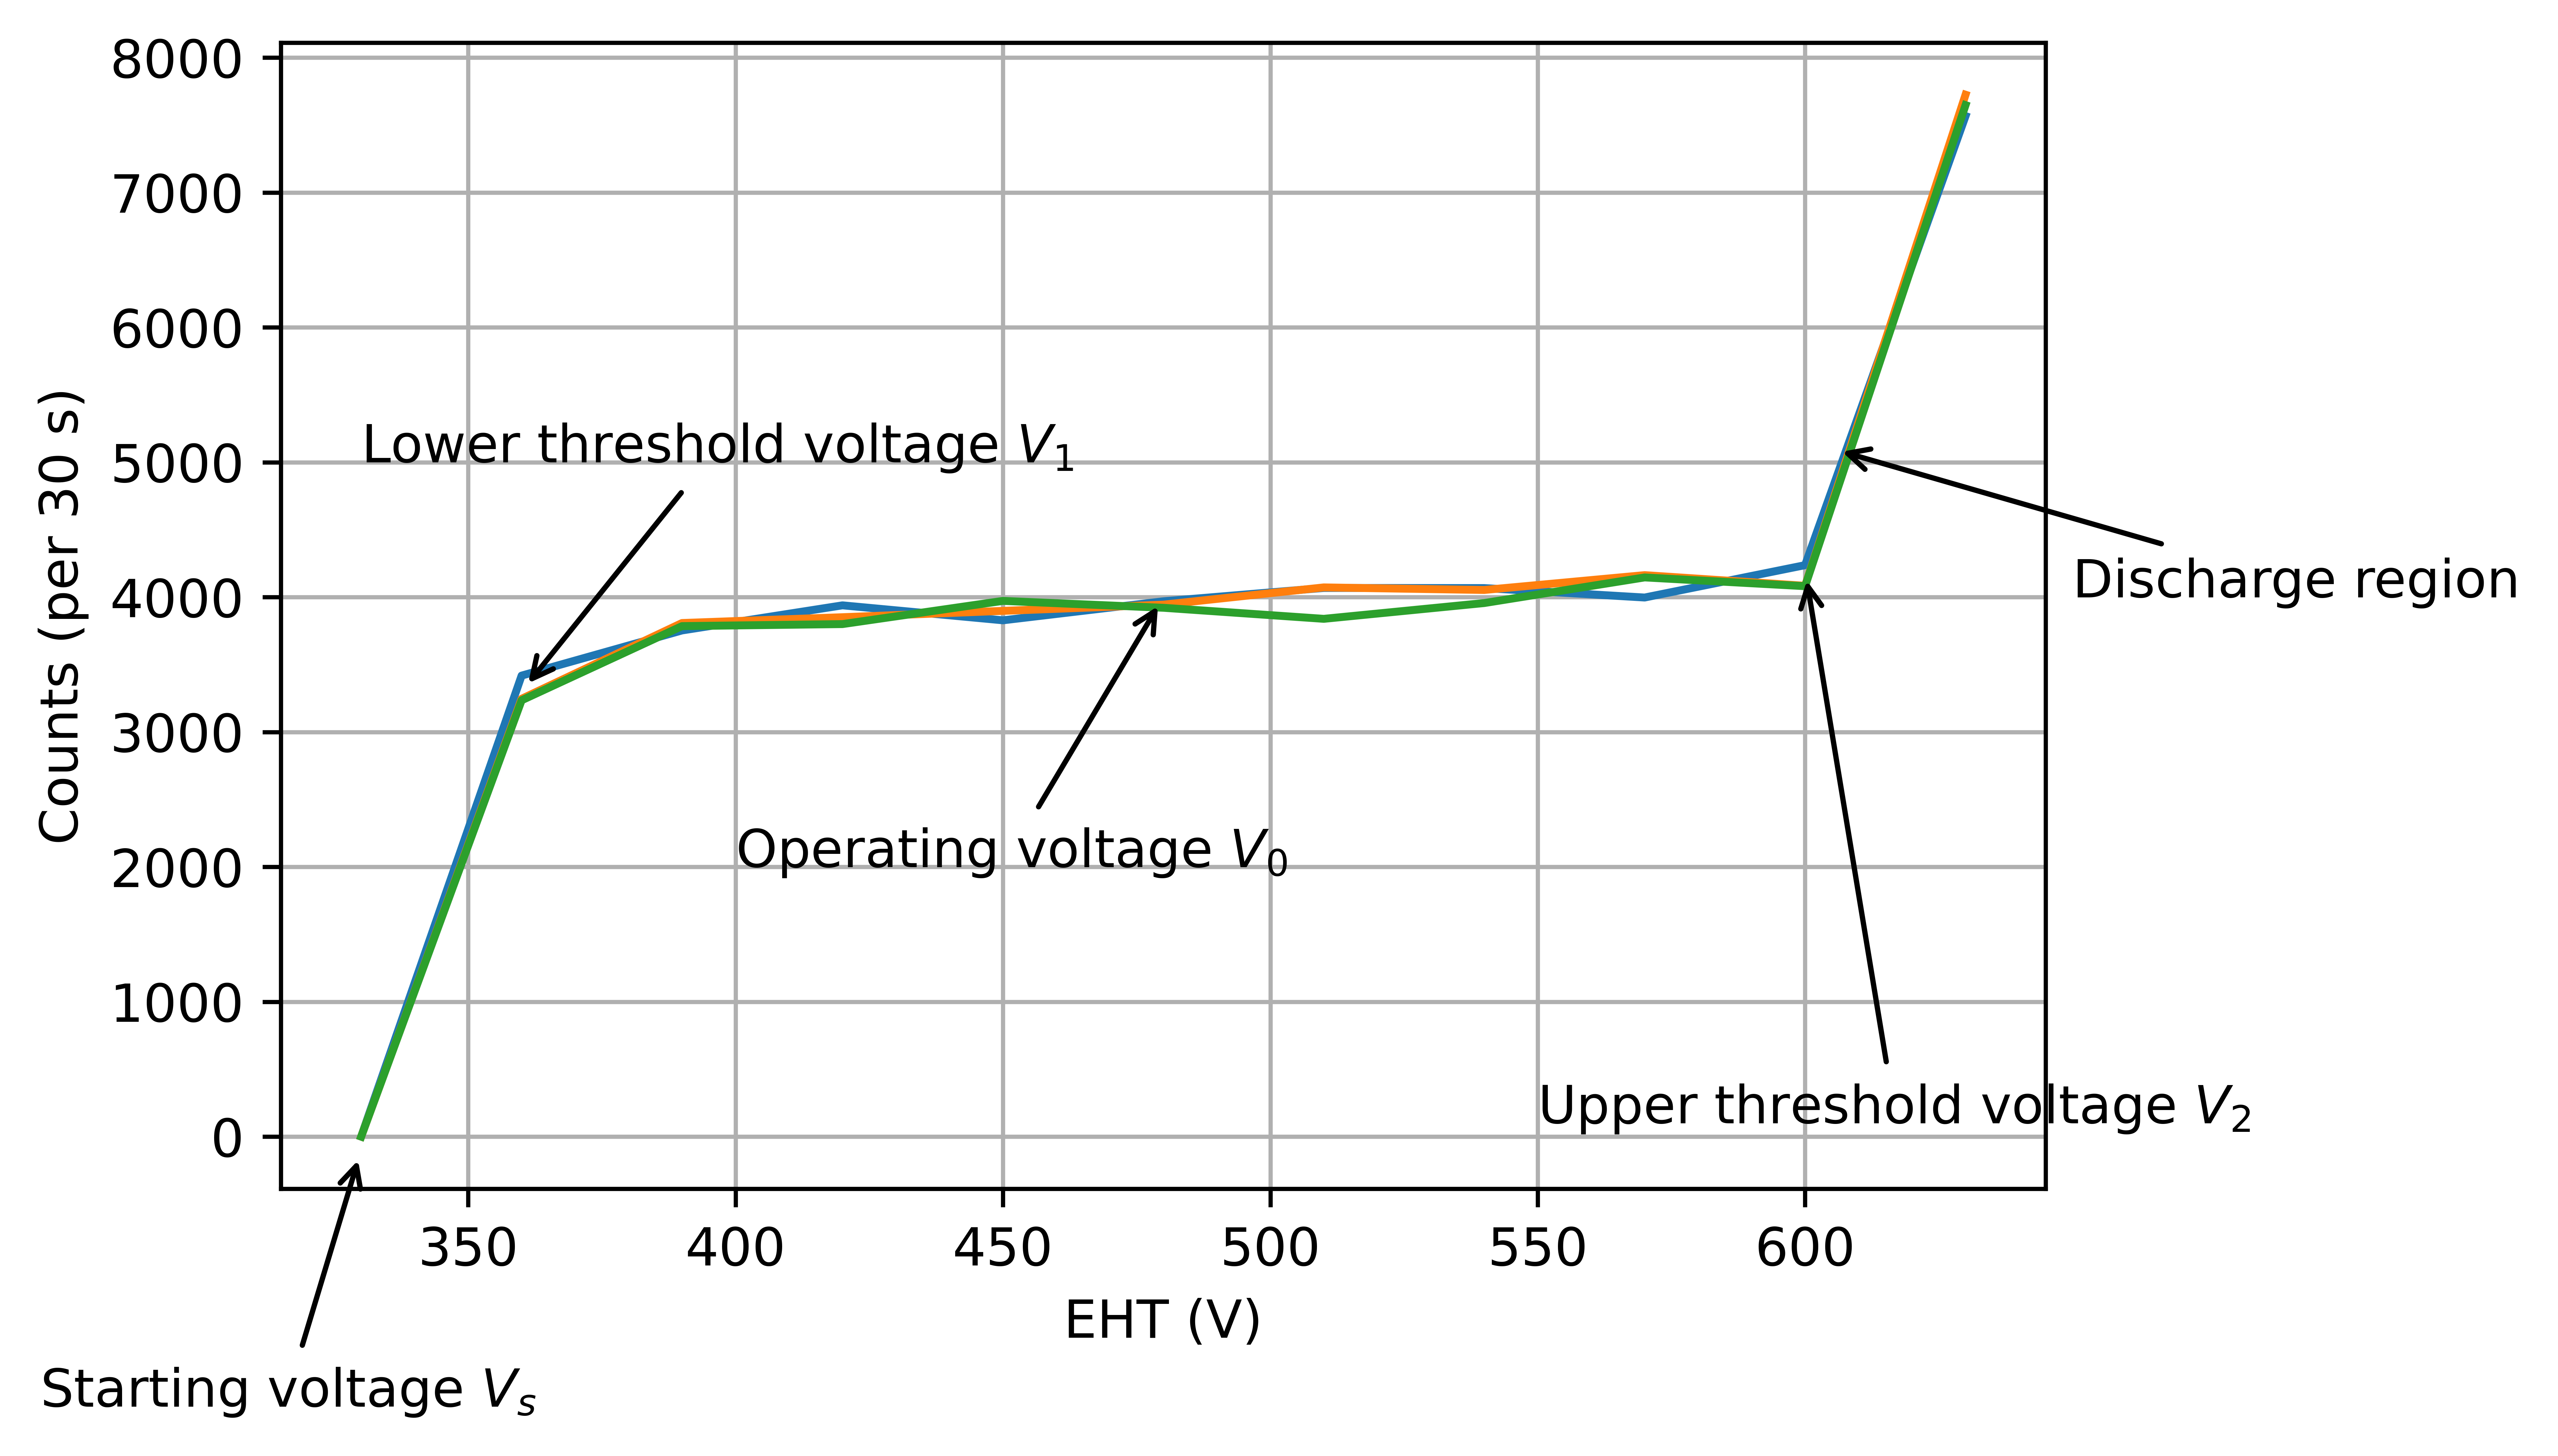
\includegraphics[scale = 0.59]{Figures/plot-GMcharac.png}
            \caption{Experimentally obtained G-M characteristics curve for Cs-137}
            \label{fig:gmcharac}
        \end{figure}
        \subsubsection{Calculations}
        From the tabulated readings (\ref{tab:GMcharac}), we have lower threshold voltage (the starting voltage of the plateau, just after the rising edge of knee), $V_1 = \SI{360}{\volt}$. Similarly, the upper threshold voltage (just before the start of the discharge region), $V_2 = \SI{600}{\volt}$. The plateau length is $VPL = V_2 - V_1 = \SI{240}{\volt}$. The operating voltage is $V_0 = \SI{480}{\volt}$. Corresponding to the three sets of data, we have three plateau slopes. The general expression of slope (expressed as  the percent change in count rate per 100 volts change in applied voltage in the plateau region) is given by
        \begin{equation}
            m = \dfrac{2 (N_2 - N_1) \times 10^4}{(N_2 + N_1)(V_2 - V_1)} \%
        \end{equation}
        where $N_1$ and $N_2$ are the count rates at the lower and the upper limits of the plateau.
        \par
        The three slopes (expressed as  the percent change in count rate per 100 volts change in applied voltage in the plateau region) so obtained are $m_1 = 8.92\%$, $m_2 = 9.53\%$ and $m_3 = 9.64\%$.
        \subsubsection{Error Analysis}
        We calculate the error found in slope as the standard deviation of $m_i$'s. The formula of standard deviation for a sample of data is
        \begin{equation}
            \sigma = \sqrt{\dfrac{\sum (x_i - \mu)^2}{N-1}}
        \end{equation}
        where $x_i$'s are the observations, $\mu$ is the mean and $N$ is the number of observations. From here we get $\sigma = 0.39\%$. The mean slope comes out to be $m = 9.36\%$.
        \subsubsection{Discussions}
        \begin{enumerate}
            \item From the plateau, it can be noticed that mid point of the characteristics of the G-M tube is defined as operating voltage and is to be used for counting applications. The tube is operated at this voltage when used in Radiation Monitors for measurements.
            \item This experiment can be repeated with Beta source by keeping the source slightly away from the end window when compared to gamma source. From this, one could notice that with Beta source, the efficiency of the detector increases.
            \item Also one can notice that with higher count rates, plateau slope increases.
        \end{enumerate}
        \subsubsection{Results}
        \begin{enumerate}
            \item The final slope (expressed as  the percent change in count rate per 100 volts change in applied voltage in the plateau region) obtained was $9.36 \pm 0.39 \%$.
            \item The slope obtained so is under $10\%$ which is desirable and well within the margin of error.
        \end{enumerate}

    
    \subsection{Inverse Square Law for Gamma rays}
        According to the inverse square law, intensity of gamma radiation falls inversely as square of the distance. The equipment required for this experiment are the G-M counting system, the end window detector stand, the G-M detector itself and a gamma source (Cs-137). The set-up arrangement is given in figure (\ref{fig:invsqsetup}).
        \begin{figure}
            \centering
            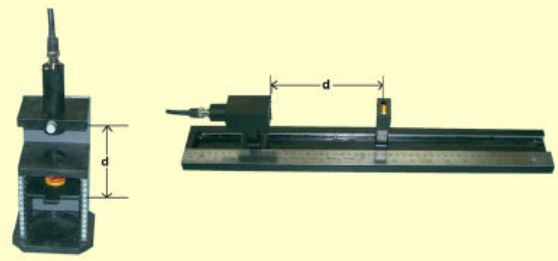
\includegraphics[scale = 0.65]{Figures/invsq.png}
            \caption{Detector, G-M stand/holder and source arrangement}
            \label{fig:invsqsetup}
        \end{figure}
        \par
        Before beginning the experiment, we take (5) readings for the background counts and compute the average background counts in 60 seconds as $(49+61+57+68+65)/5 = 60$. The operating voltage, as determined in first experiment (\ref{sec:GMtubecharac}), is $V_0 = \SI{480}{\volt}$.
        \begin{table*}[]
        \caption{Readings for the inverse square law experiment}
        \label{tab:invsq}
        \setlength{\tabcolsep}{15pt}
        \begin{tabular}{@{}cccccc@{}}
        \toprule
          \begin{tabular}[c]{@{}c@{}}\textbf{Distance}, $d$  \\  (cm)\end{tabular} &
          \begin{tabular}[c]{@{}c@{}}\textbf{Counts}               \\ (60 s)\end{tabular} &
          \begin{tabular}[c]{@{}c@{}}\textbf{Corrected counts}\\ (60 s)\end{tabular} &
          \begin{tabular}[c]{@{}c@{}}\textbf{Net count rate}, $R$\\ ($s^{-1}$)\end{tabular} &
          \begin{tabular}[c]{@{}c@{}}\textbf{Product}\\ ($C = Rd^2$)\end{tabular} &
          \begin{tabular}[c]{@{}c@{}}\textbf{Transformation}\\ ($1/d^2$ in $1/m^2$)\end{tabular} \\ \midrule
        2   & 4409 & 4349 & 72.48 & 290 & 2500 \\
        2.5 & 3698 & 3638 & 60.63 & 379 & 1600 \\
        3   & 2955 & 2895 & 48.25 & 434 & 1111 \\
        3.5 & 2527 & 2467 & 41.12 & 504 & 816  \\
        4   & 2162 & 2102 & 35.03 & 561 & 625  \\
        4.5 & 1743 & 1683 & 28.05 & 568 & 494  \\
        5   & 1514 & 1454 & 24.23 & 606 & 400  \\
        5.5 & 1332 & 1272 & 21.20 & 641 & 331  \\
        6   & 1102 & 1042 & 17.37 & 625 & 278  \\
        6.5 & 1019 & 959  & 15.98 & 675 & 237  \\
        7   & 888  & 828  & 13.80 & 676 & 204  \\ \bottomrule
        \end{tabular}
        \end{table*}
        \begin{figure}
            \centering
            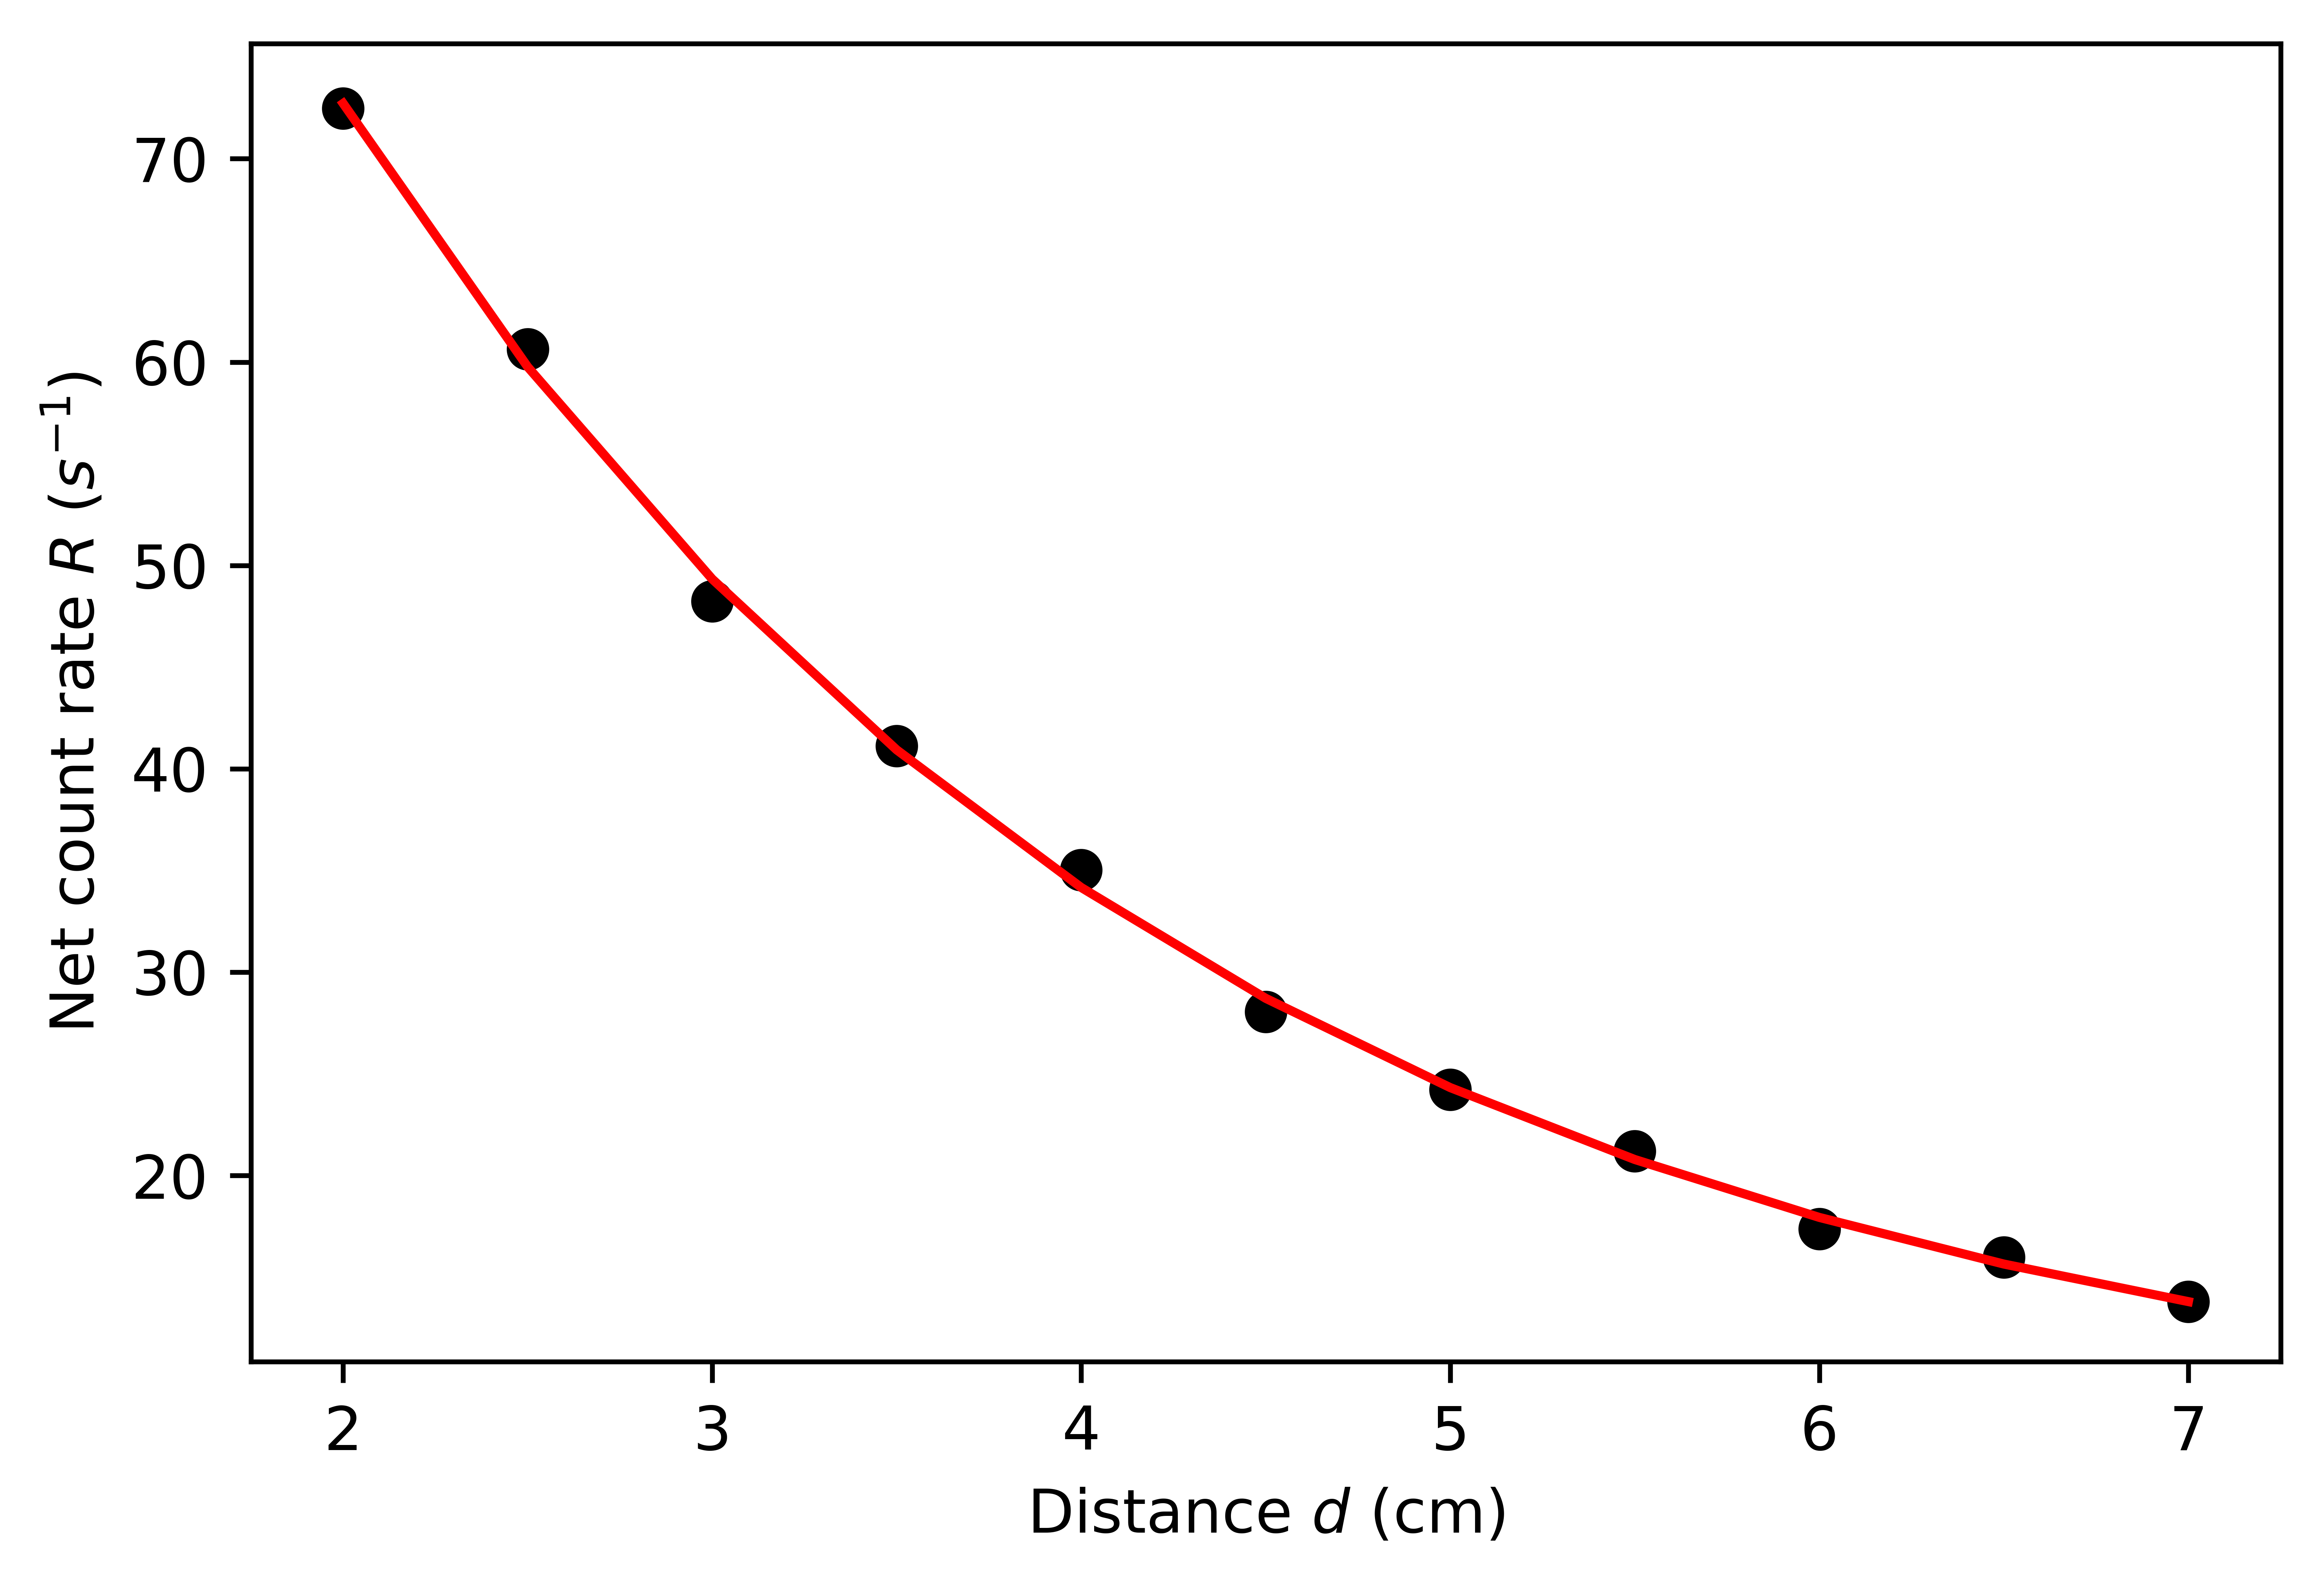
\includegraphics[scale = 0.63]{Figures/plot-invsq-1.png}
            \caption{Plot of net count rate $R$ against distance $d$}
            \label{fig:invsq-1}
        \end{figure}
        \begin{figure}
            \centering
            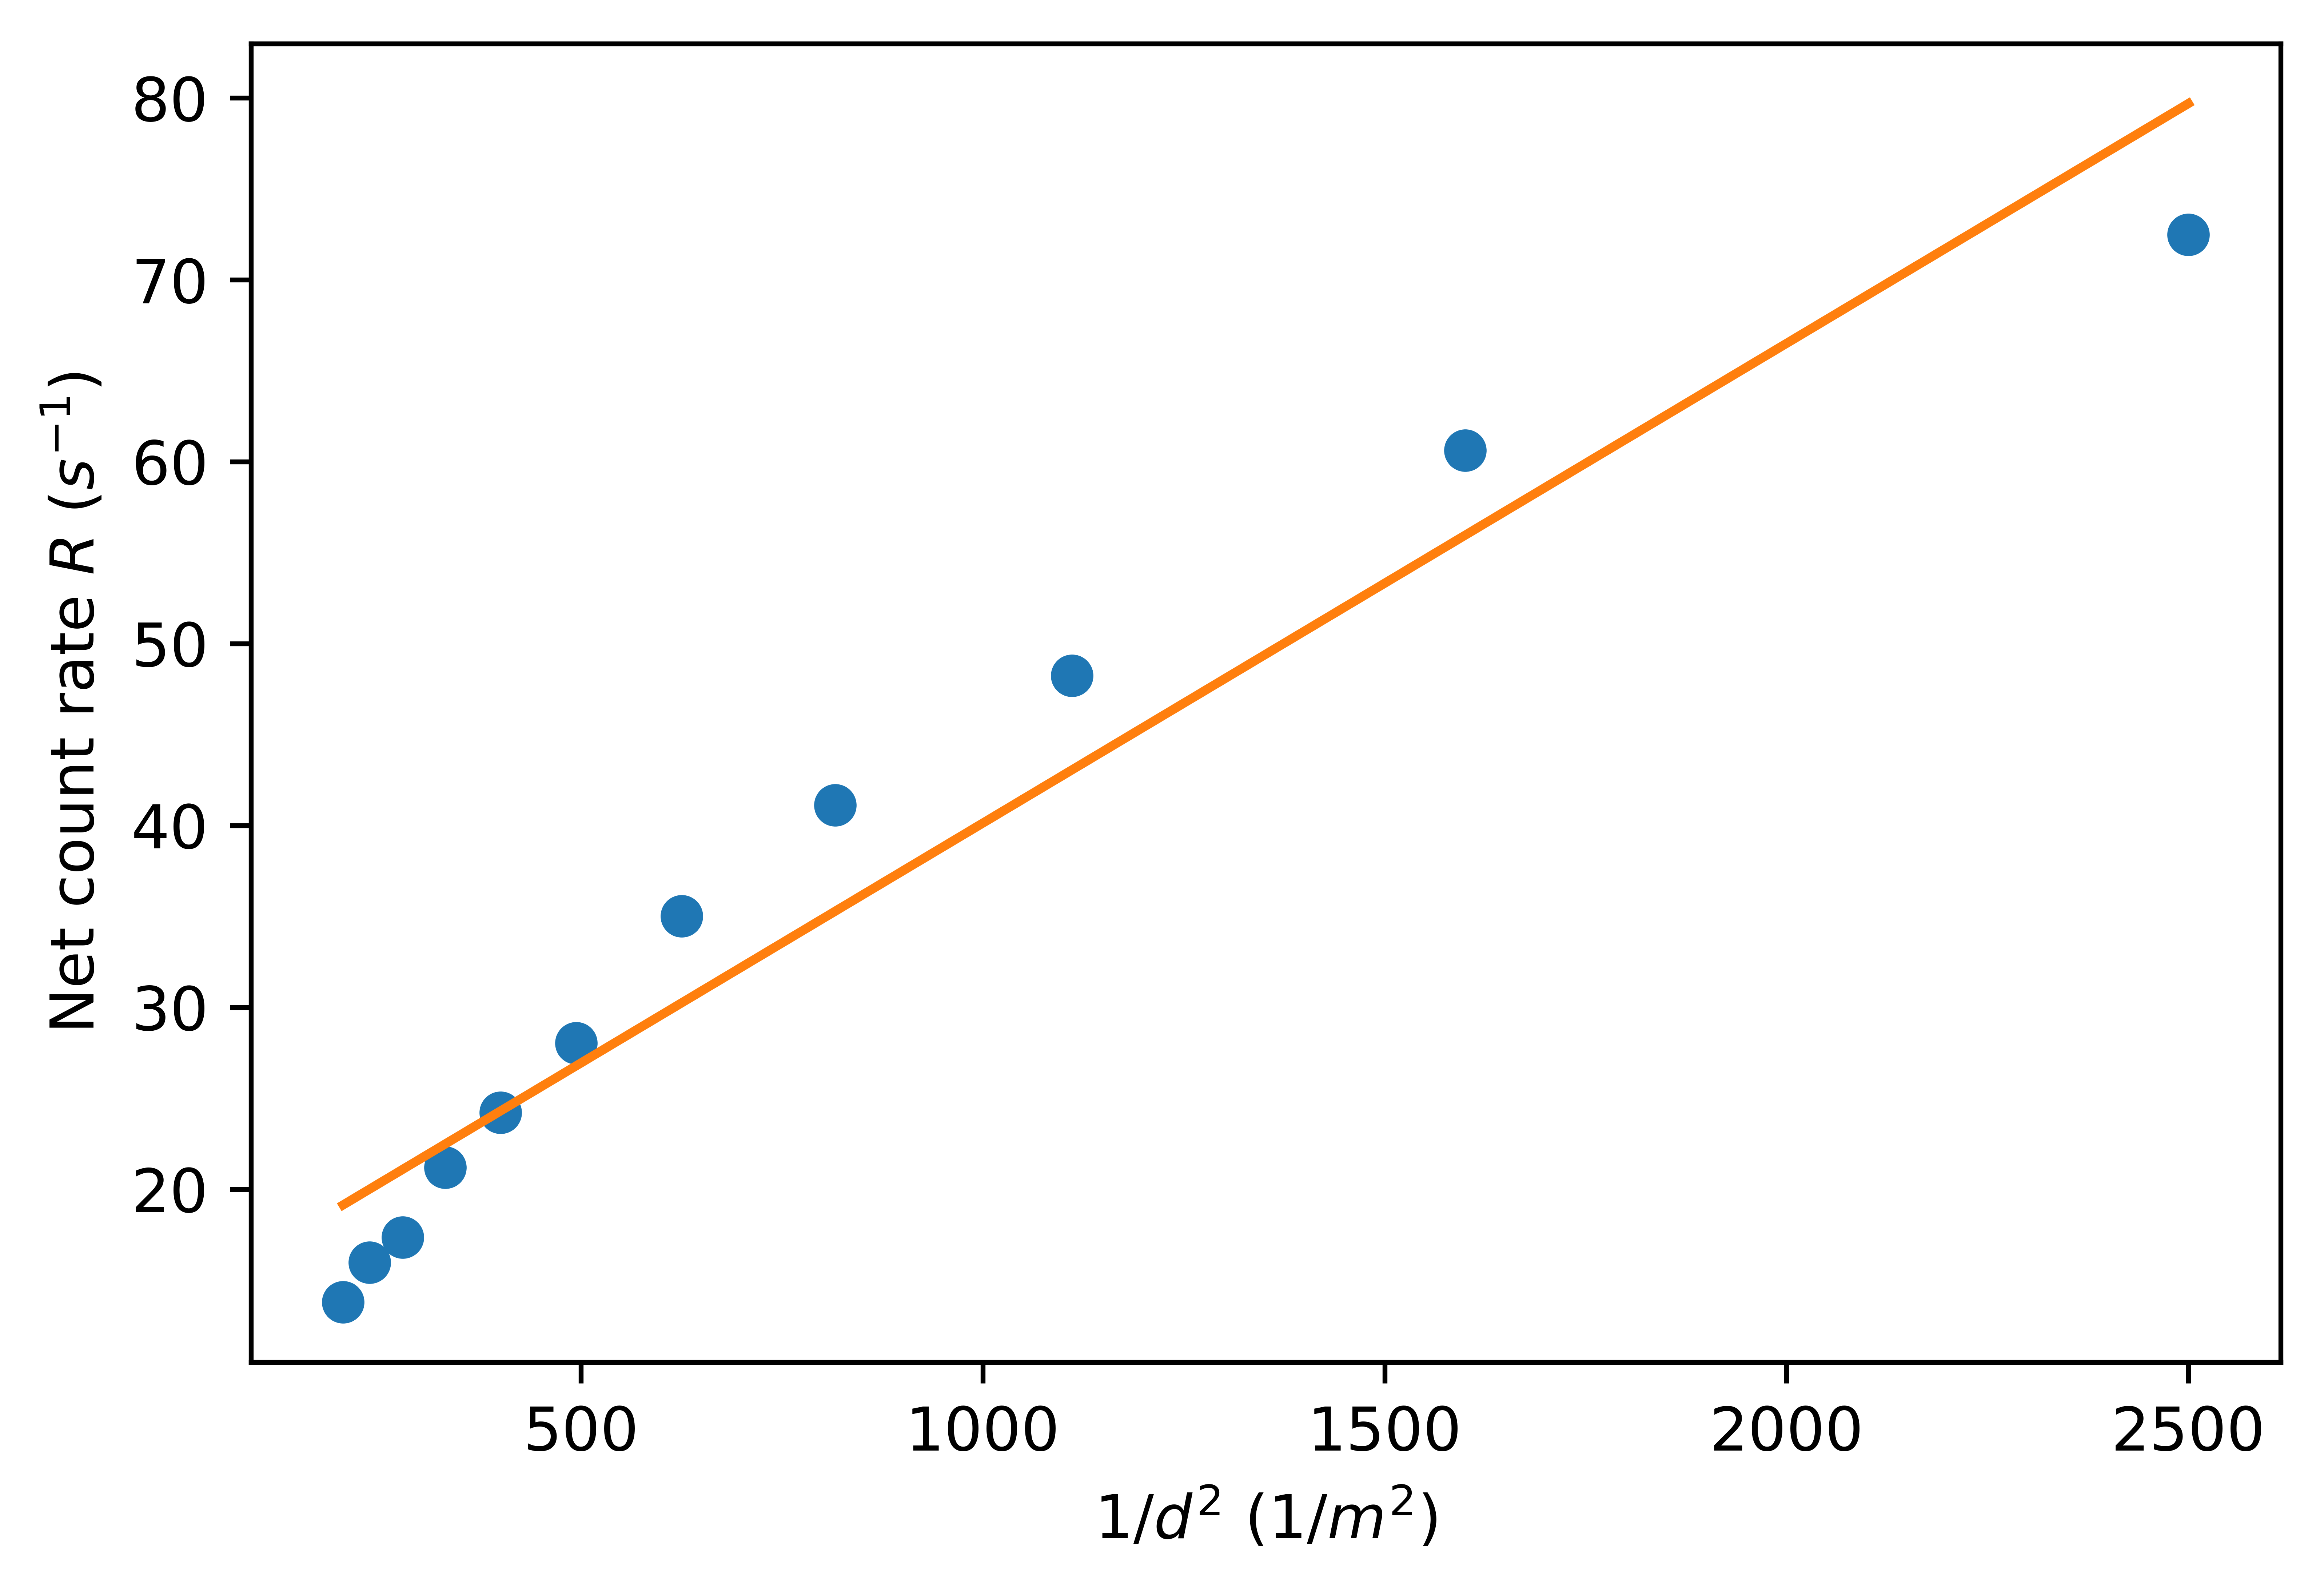
\includegraphics[scale = 0.63]{Figures/plot-invsq-2.png}
            \caption{Plot of net count rate $R$ against inverse of distance square $1/d^2$}
            \label{fig:invsq-2}
        \end{figure}
        \begin{table}[]
        \caption{The $\log d$ and $\log R$ values for inverse square law experiment}
        \label{tab:invsqlog}
        \setlength{\tabcolsep}{10pt}
        \begin{tabular}{@{}cccc@{}}
        \toprule
        \begin{tabular}[c]{@{}c@{}}\textbf{Distance}, $d$   \\ (cm)\end{tabular} & $\log d$ & \begin{tabular}[c]{@{}c@{}}\textbf{Net count rate}, $R$\\ ($s^{-1}$)\end{tabular} & $\log R$ \\ \midrule
        2   & 0.301 & 72.48 & 1.860 \\
        2.5 & 0.398 & 60.63 & 1.783 \\
        3   & 0.477 & 48.25 & 1.683 \\
        3.5 & 0.544 & 41.12 & 1.614 \\
        4   & 0.602 & 35.03 & 1.544 \\
        4.5 & 0.653 & 28.05 & 1.448 \\
        5   & 0.699 & 24.23 & 1.384 \\
        5.5 & 0.740 & 21.20 & 1.326 \\
        6   & 0.778 & 17.37 & 1.240 \\
        6.5 & 0.813 & 15.98 & 1.204 \\
        7   & 0.845 & 13.80 & 1.140 \\ \bottomrule
        \end{tabular}
        \end{table}
        \begin{figure}
            \centering
            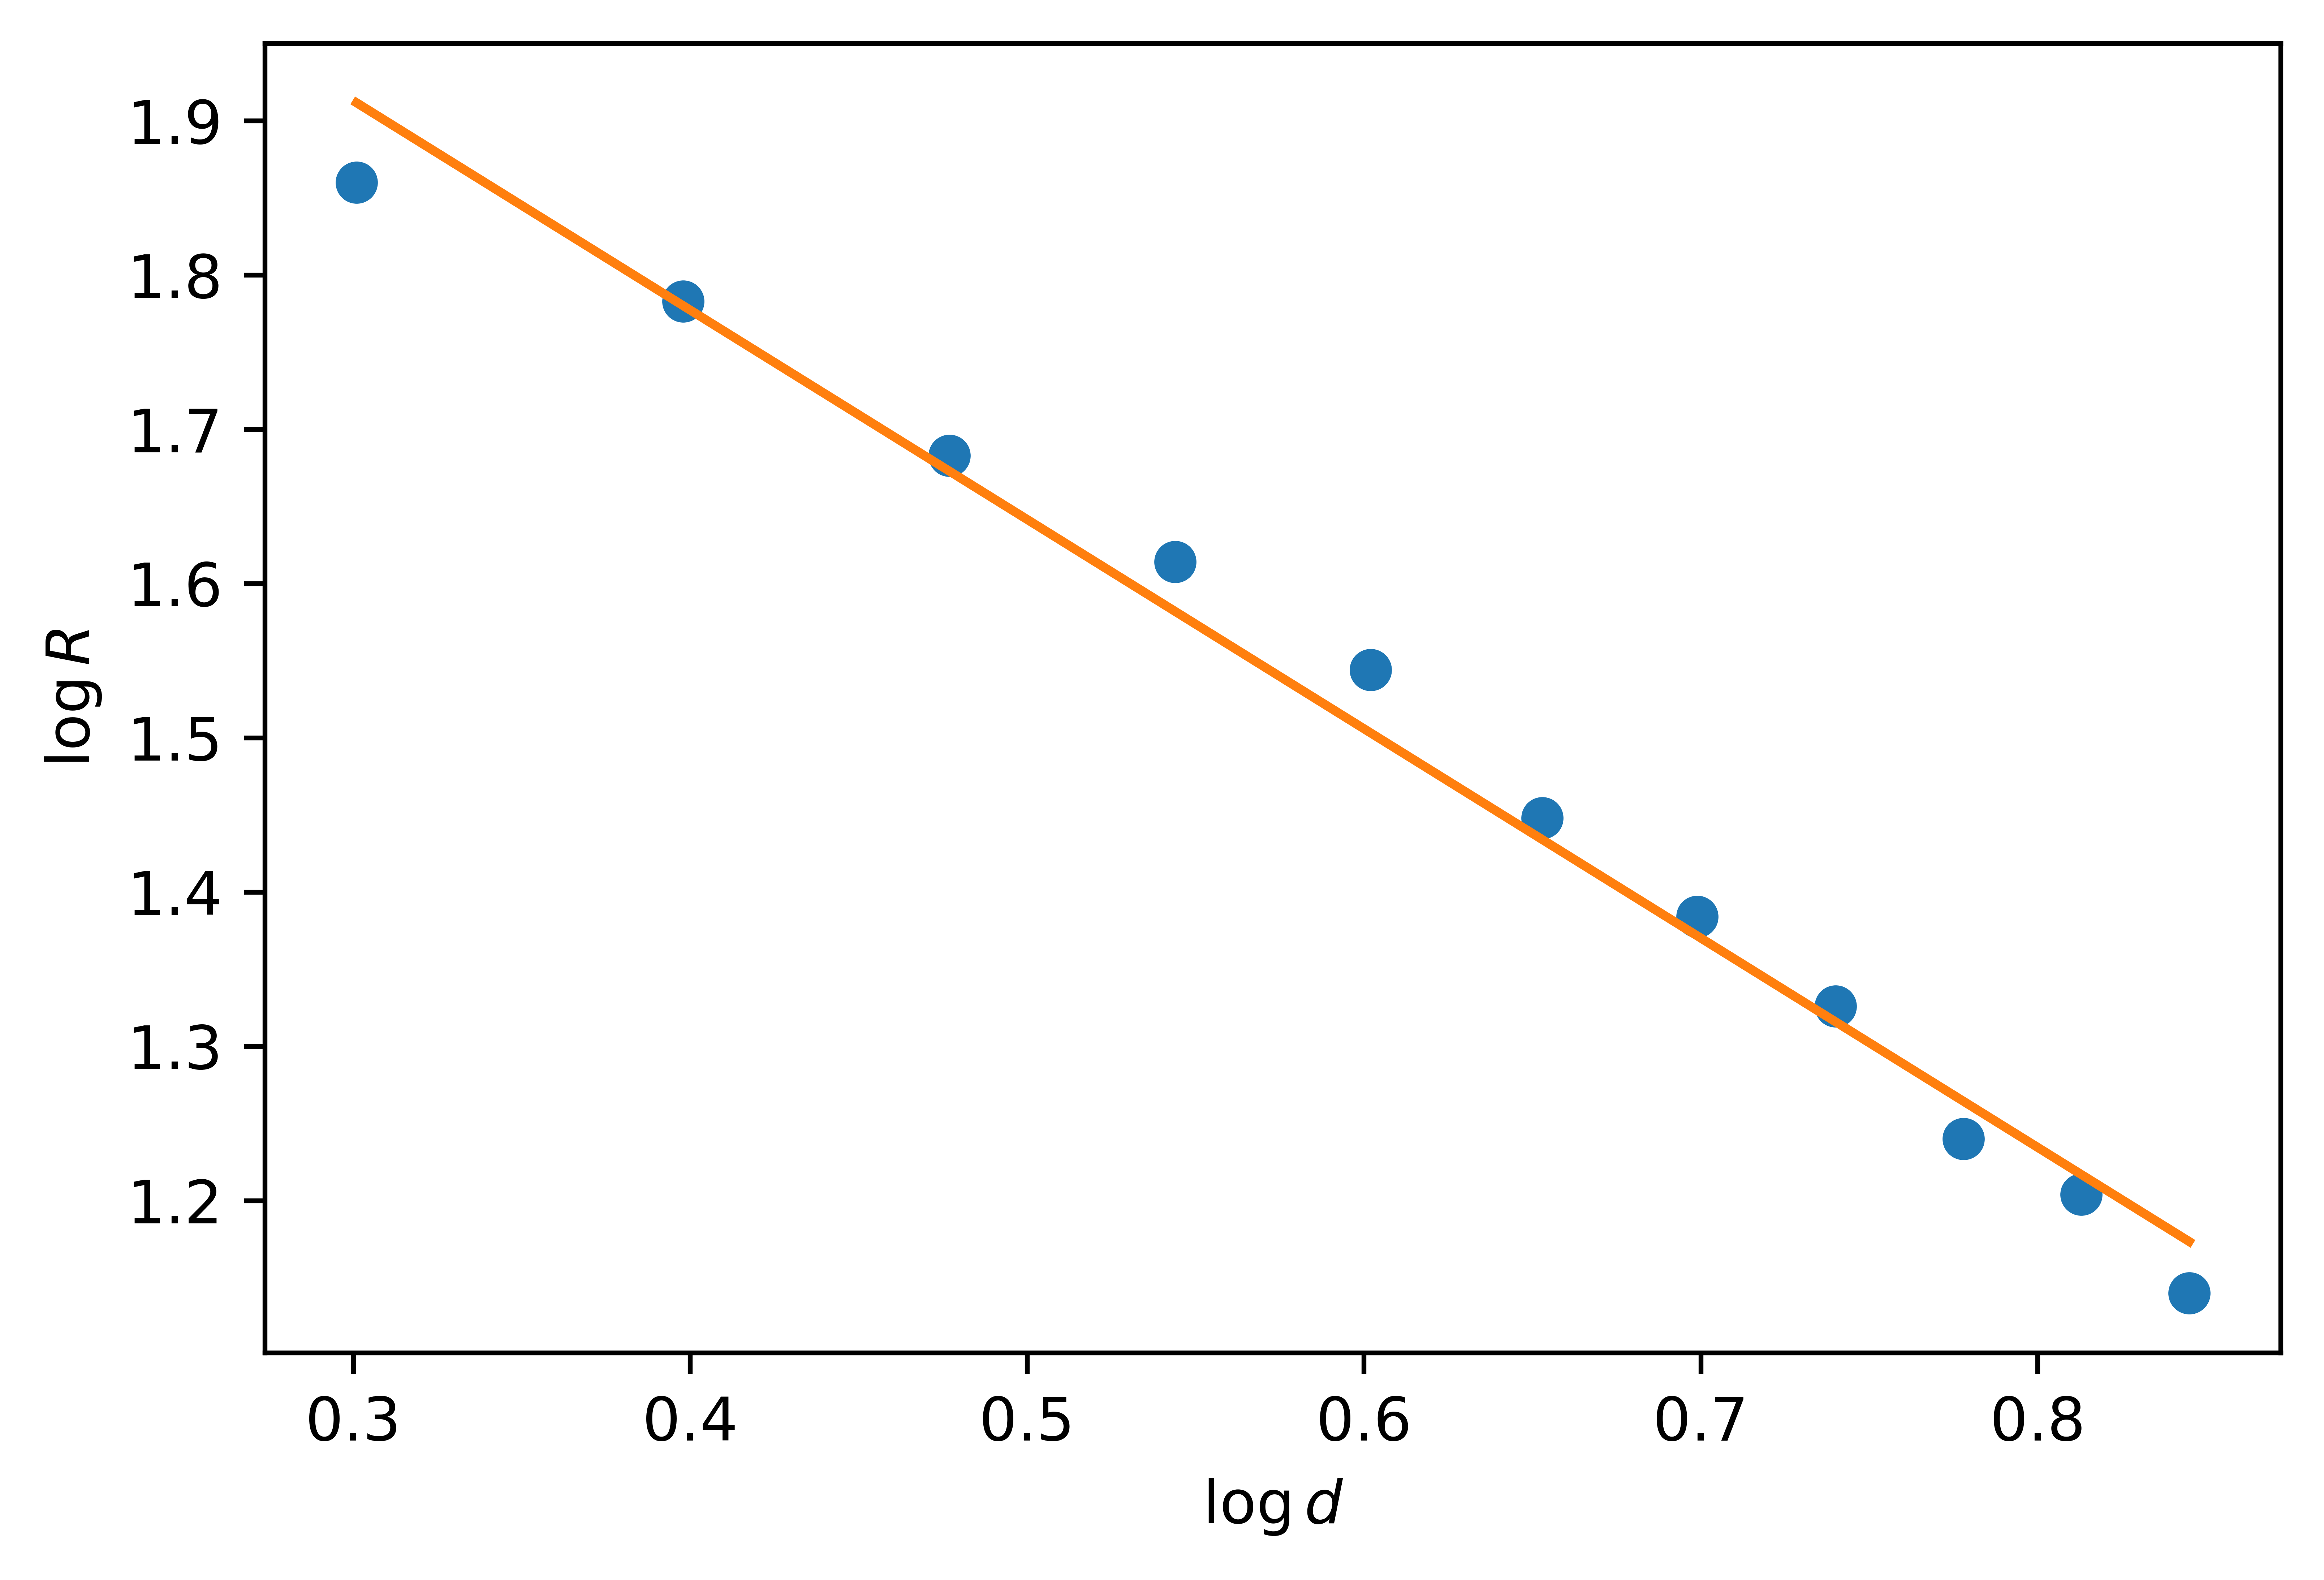
\includegraphics[scale = 0.63]{Figures/plot-invsq-3.png}
            \caption{Plot of $\log R$ against $\log d$}
            \label{fig:invsq-3}
        \end{figure}
        \subsubsection{Data Analysis}
        If the count rate obeys the inverse square law, it can be easily be shown that the product $C = R d^2$ is a constant. The results of the product ($Rd^2$) are shown in the table above; allowing for statistical fluctuations, the results obey this law, with a mean value of $C = 542$. Then the observed net count rate as a function of distance is given by
        \begin{equation}
            R_d = \dfrac{542}{d^2}
        \end{equation}
        \par
        An alternative analysis method involves transforming the data so that the results lie on a straight line. For this purpose \textit{Net Count Rate} ($R$) Vs. \textit{Reciprocal of the distance square} ($1/d^2$) are plotted (figure (\ref{fig:invsq-2})). This will be a straight line passing through the origin $(0, 0)$ as this point corresponds to a source-detector distance of infinity. Gradient can be estimated easily from the \textit{Net Count Rate} ($R$) corresponding to a value of ($1/d^2$).
        \par
        Another way of data analysis is by plotting these values on a log-log graph sheet or compute log values and plot them on a linear graph sheet (\ref{fig:invsq-3}). 
        \subsubsection{Discussions}
        \begin{enumerate}
            \item Gamma radiation is part of the electromagnetic spectrum. It is not absorbed by the air, but its intensity decreases because it spreads out. Therefore, the intensity varies with the inverse square of distance: it follows an inverse square law.
            \item This is the same law that governs all electromagnetic radiation (like the Sun's luminosity). This is some evidence that gamma radiation is part of the electromagnetic spectrum.
            \item In order to protect yourself from gamma radiation the best thing to do is to move farther away. At 10 times the distance you will be 100 times as safe.
        \end{enumerate}
        \subsubsection{Results}
        \begin{enumerate}
            \item The plot between net count rate and distance was expectedly obtained as an exponentially decreasing curve.
            \item The plot between net count rate and inverse square of distance was expectedly obtained as a straight line curve (with a positive slope).
            \item The log-log plot between net count rate and distance was expectedly obtained as a straight line curve (with a negative slope).
        \end{enumerate}


    \subsection{Nuclear Counting Statistics}
        Radioactive decay is a random process. Consequently, any measurement based on observing the radiation emitted in a nuclear decay is subject to some degree of statistical fluctuations. These inherent fluctuations are unavoidable in all nuclear measurements. The term counting statistics includes the framework of statistical analysis required to process the results of nuclear counting experiments and to make predictions about the expected precision of quantities derived from these measurements.
        \par
        Although each measurement (number of decays in a given interval) for a radioactive sample is independent of all previous measurements (due to randomness of the process), for a large number of individual measurements the deviation of the individual count rates from the average count rate behaves in a predictable manner. Small deviations from the average are much more likely than large deviations. These statistical fluctuations in the nuclear decay can be understood from the statistical models utilizing Poisson distribution or Gaussian (Normal) distribution. If we observe a given radioactive nucleus for a time $t$ and define the success as ``the nucleus decays during the process'' then the probability of success $p$ is given by ($1-e^{-\lambda t}$). The Poisson distribution applies when the success probability $p$ is small and the number successes (i.e. number of counts measured) is also small (say $<30$). In practical terms, this condition implies that we have chosen an observation time that is small compared with the half-life of the source. When the average number of the number of successes becomes relatively large (say $> 30$) we can utilize the Gaussian model of distribution. Since in most of the cases the count rates are reasonably large (few tens of counts per second) the Gaussian model has become widely applicable to many problems in counting statistics. On the other hand the Poisson distribution is applicable in the case of background counts.
        \par
        The Poisson distribution function is given by
        \begin{equation}
            P(N) = \dfrac{\overline{N}^N e^{-\overline{N}}}{N!}
        \end{equation}
        where $\overline{N}$ is the experimental mean. The corresponding standard deviation is given by $\sigma_p = \sqrt{\overline{N}}$. 
        \par
        The Gaussian distribution function is given by
        \begin{equation}
            P(N) = \dfrac{1}{\sqrt{2 \pi \overline{N}}} \exp \Bigg({- \dfrac{(N - \overline{N})^2}{2 \overline{N}}} \Bigg)
        \end{equation}
        Here the standard deviation is given by $\sigma_G = \sqrt{\overline{N}}$.
        \par
        The equipment required for this experiment are the G-M counting system, the end window detector stand, the G-M detector itself and a radioactive source.
        \begin{table*}[]
        \caption{Nuclear Counting Statistics}
        \label{tab:my-table}
        \setlength{\tabcolsep}{12pt}
        \begin{tabular}{@{}cccc@{}}
        \toprule
        \textbf{Background Counts} & \textbf{Poisson Distribution value} & \textbf{Counts with source} & \textbf{Gaussian distribution value} \\ \midrule
        4         & 0.0539  & 1230               & 0.0006   \\
        4         & 0.0539  & 1269               & 0.0045   \\
        4         & 0.0539  & 1273               & 0.0052   \\
        5         & 0.0875  & 1275               & 0.0056   \\
        5         & 0.0875  & 1278               & 0.0061   \\
        5         & 0.0875  & 1281               & 0.0067   \\
        5         & 0.0875  & 1281               & 0.0067   \\
        6         & 0.1184  & 1287               & 0.0077   \\
        6         & 0.1184  & 1289               & 0.0081   \\
        6         & 0.1184  & 1293               & 0.0088   \\
        6         & 0.1184  & 1293               & 0.0088   \\
        6         & 0.1184  & 1294               & 0.0089   \\
        6         & 0.1184  & 1299               & 0.0097   \\
        6         & 0.1184  & 1300               & 0.0098   \\
        6         & 0.1184  & 1300               & 0.0098   \\
        6         & 0.1184  & 1304               & 0.0103   \\
        7         & 0.1374  & 1305               & 0.0104   \\
        7         & 0.1374  & 1305               & 0.0104   \\
        7         & 0.1374  & 1308               & 0.0106   \\
        7         & 0.1374  & 1308               & 0.0106   \\
        7         & 0.1374  & 1309               & 0.0107   \\
        7         & 0.1374  & 1309               & 0.0107   \\
        8         & 0.1395  & 1311               & 0.0108   \\
        8         & 0.1395  & 1315               & 0.0110   \\
        8         & 0.1395  & 1316               & 0.0110   \\
        8         & 0.1395  & 1317               & 0.0110   \\
        8         & 0.1395  & 1320               & 0.0110   \\
        9         & 0.1258  & 1320               & 0.0110   \\
        9         & 0.1258  & 1320               & 0.0110   \\
        9         & 0.1258  & 1321               & 0.0109   \\
        9         & 0.1258  & 1322               & 0.0109   \\
        9         & 0.1258  & 1323               & 0.0109   \\
        9         & 0.1258  & 1327               & 0.0106   \\
        9         & 0.1258  & 1327               & 0.0106   \\
        9         & 0.1258  & 1328               & 0.0105   \\
        9         & 0.1258  & 1333               & 0.0100   \\
        9         & 0.1258  & 1337               & 0.0095   \\
        9         & 0.1258  & 1339               & 0.0092   \\
        10        & 0.1022  & 1343               & 0.0086   \\
        10        & 0.1022  & 1345               & 0.0082   \\
        10        & 0.1022  & 1347               & 0.0079   \\
        10        & 0.1022  & 1349               & 0.0075   \\
        11        & 0.0754  & 1349               & 0.0075   \\
        11        & 0.0754  & 1351               & 0.0072   \\
        12        & 0.0510  & 1355               & 0.0064   \\
        12        & 0.0510  & 1358               & 0.0059   \\
        12        & 0.0510  & 1358               & 0.0059   \\
        13        & 0.0319  & 1376               & 0.0030   \\
        13        & 0.0319  & 1384               & 0.0020   \\
        15        & 0.0100  & 1387               & 0.0017   \\ \bottomrule
        \end{tabular}
        \end{table*}
        \begin{figure}
            \centering
            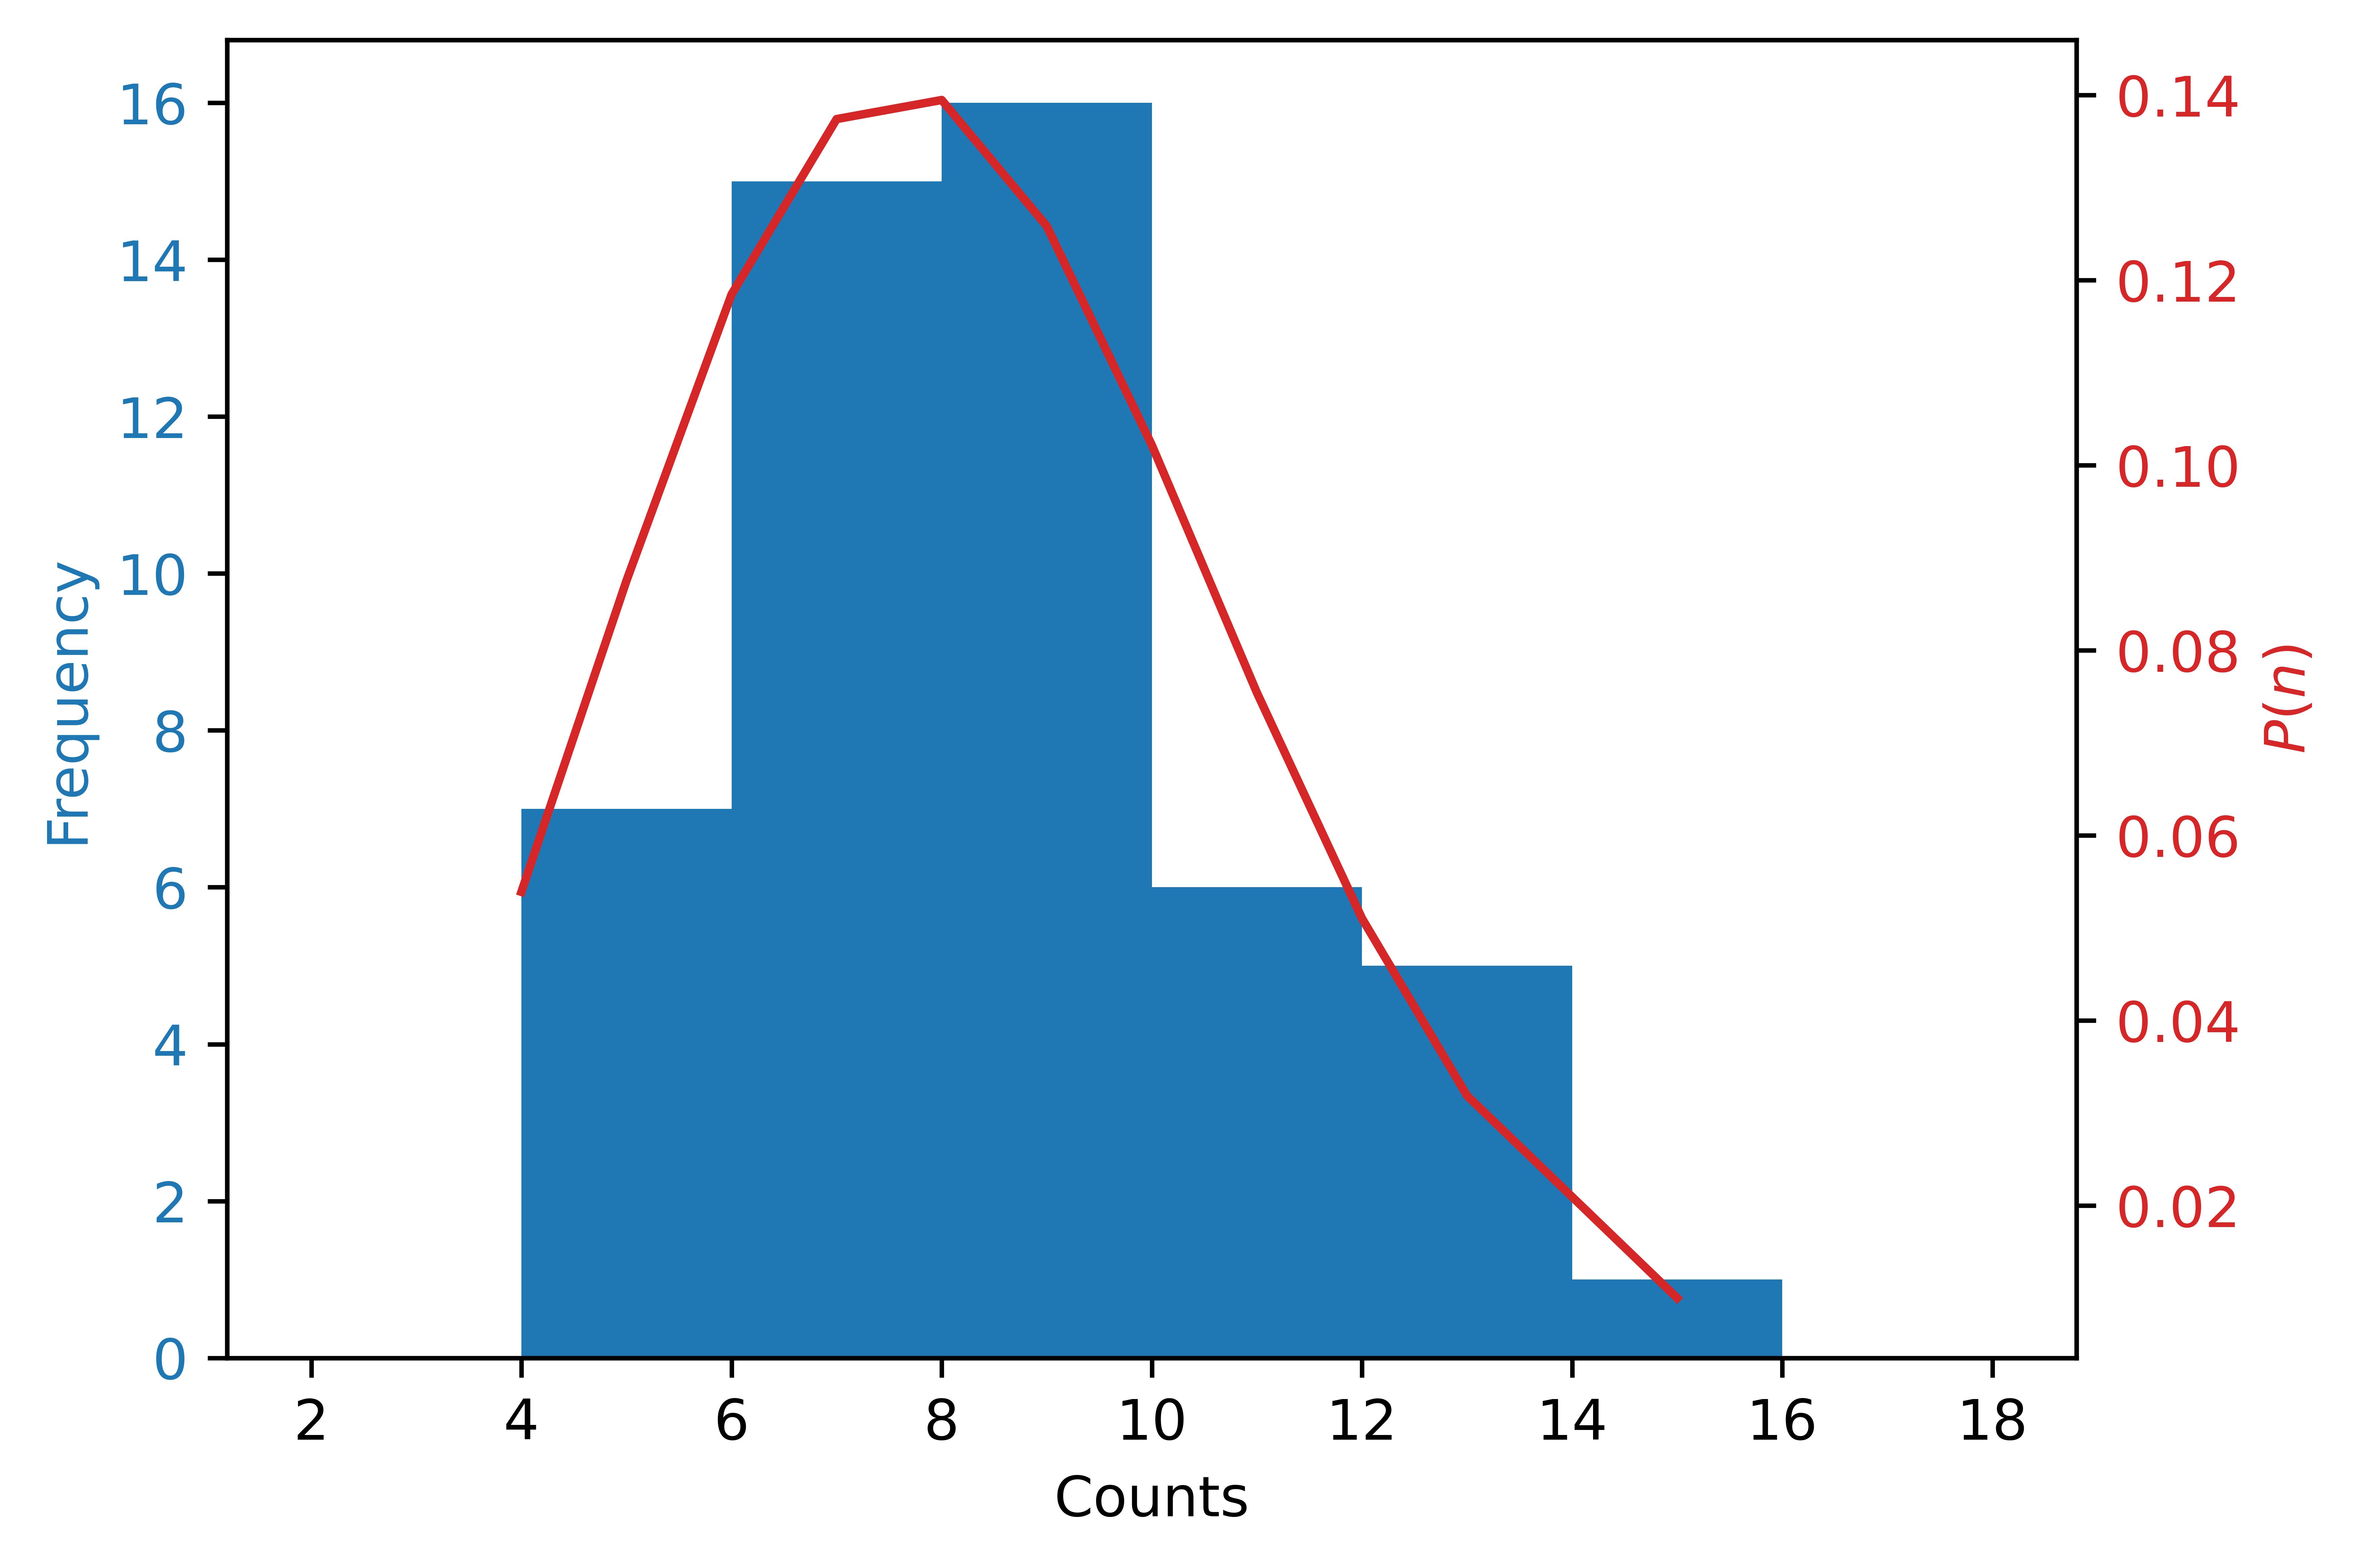
\includegraphics[scale = 0.63]{Figures/plot-ncs-bg.png}
            \caption{Histogram for background counts and overlaid Poisson curve}
            \label{fig:ncs-bg}
        \end{figure}
        \begin{figure}
            \centering
            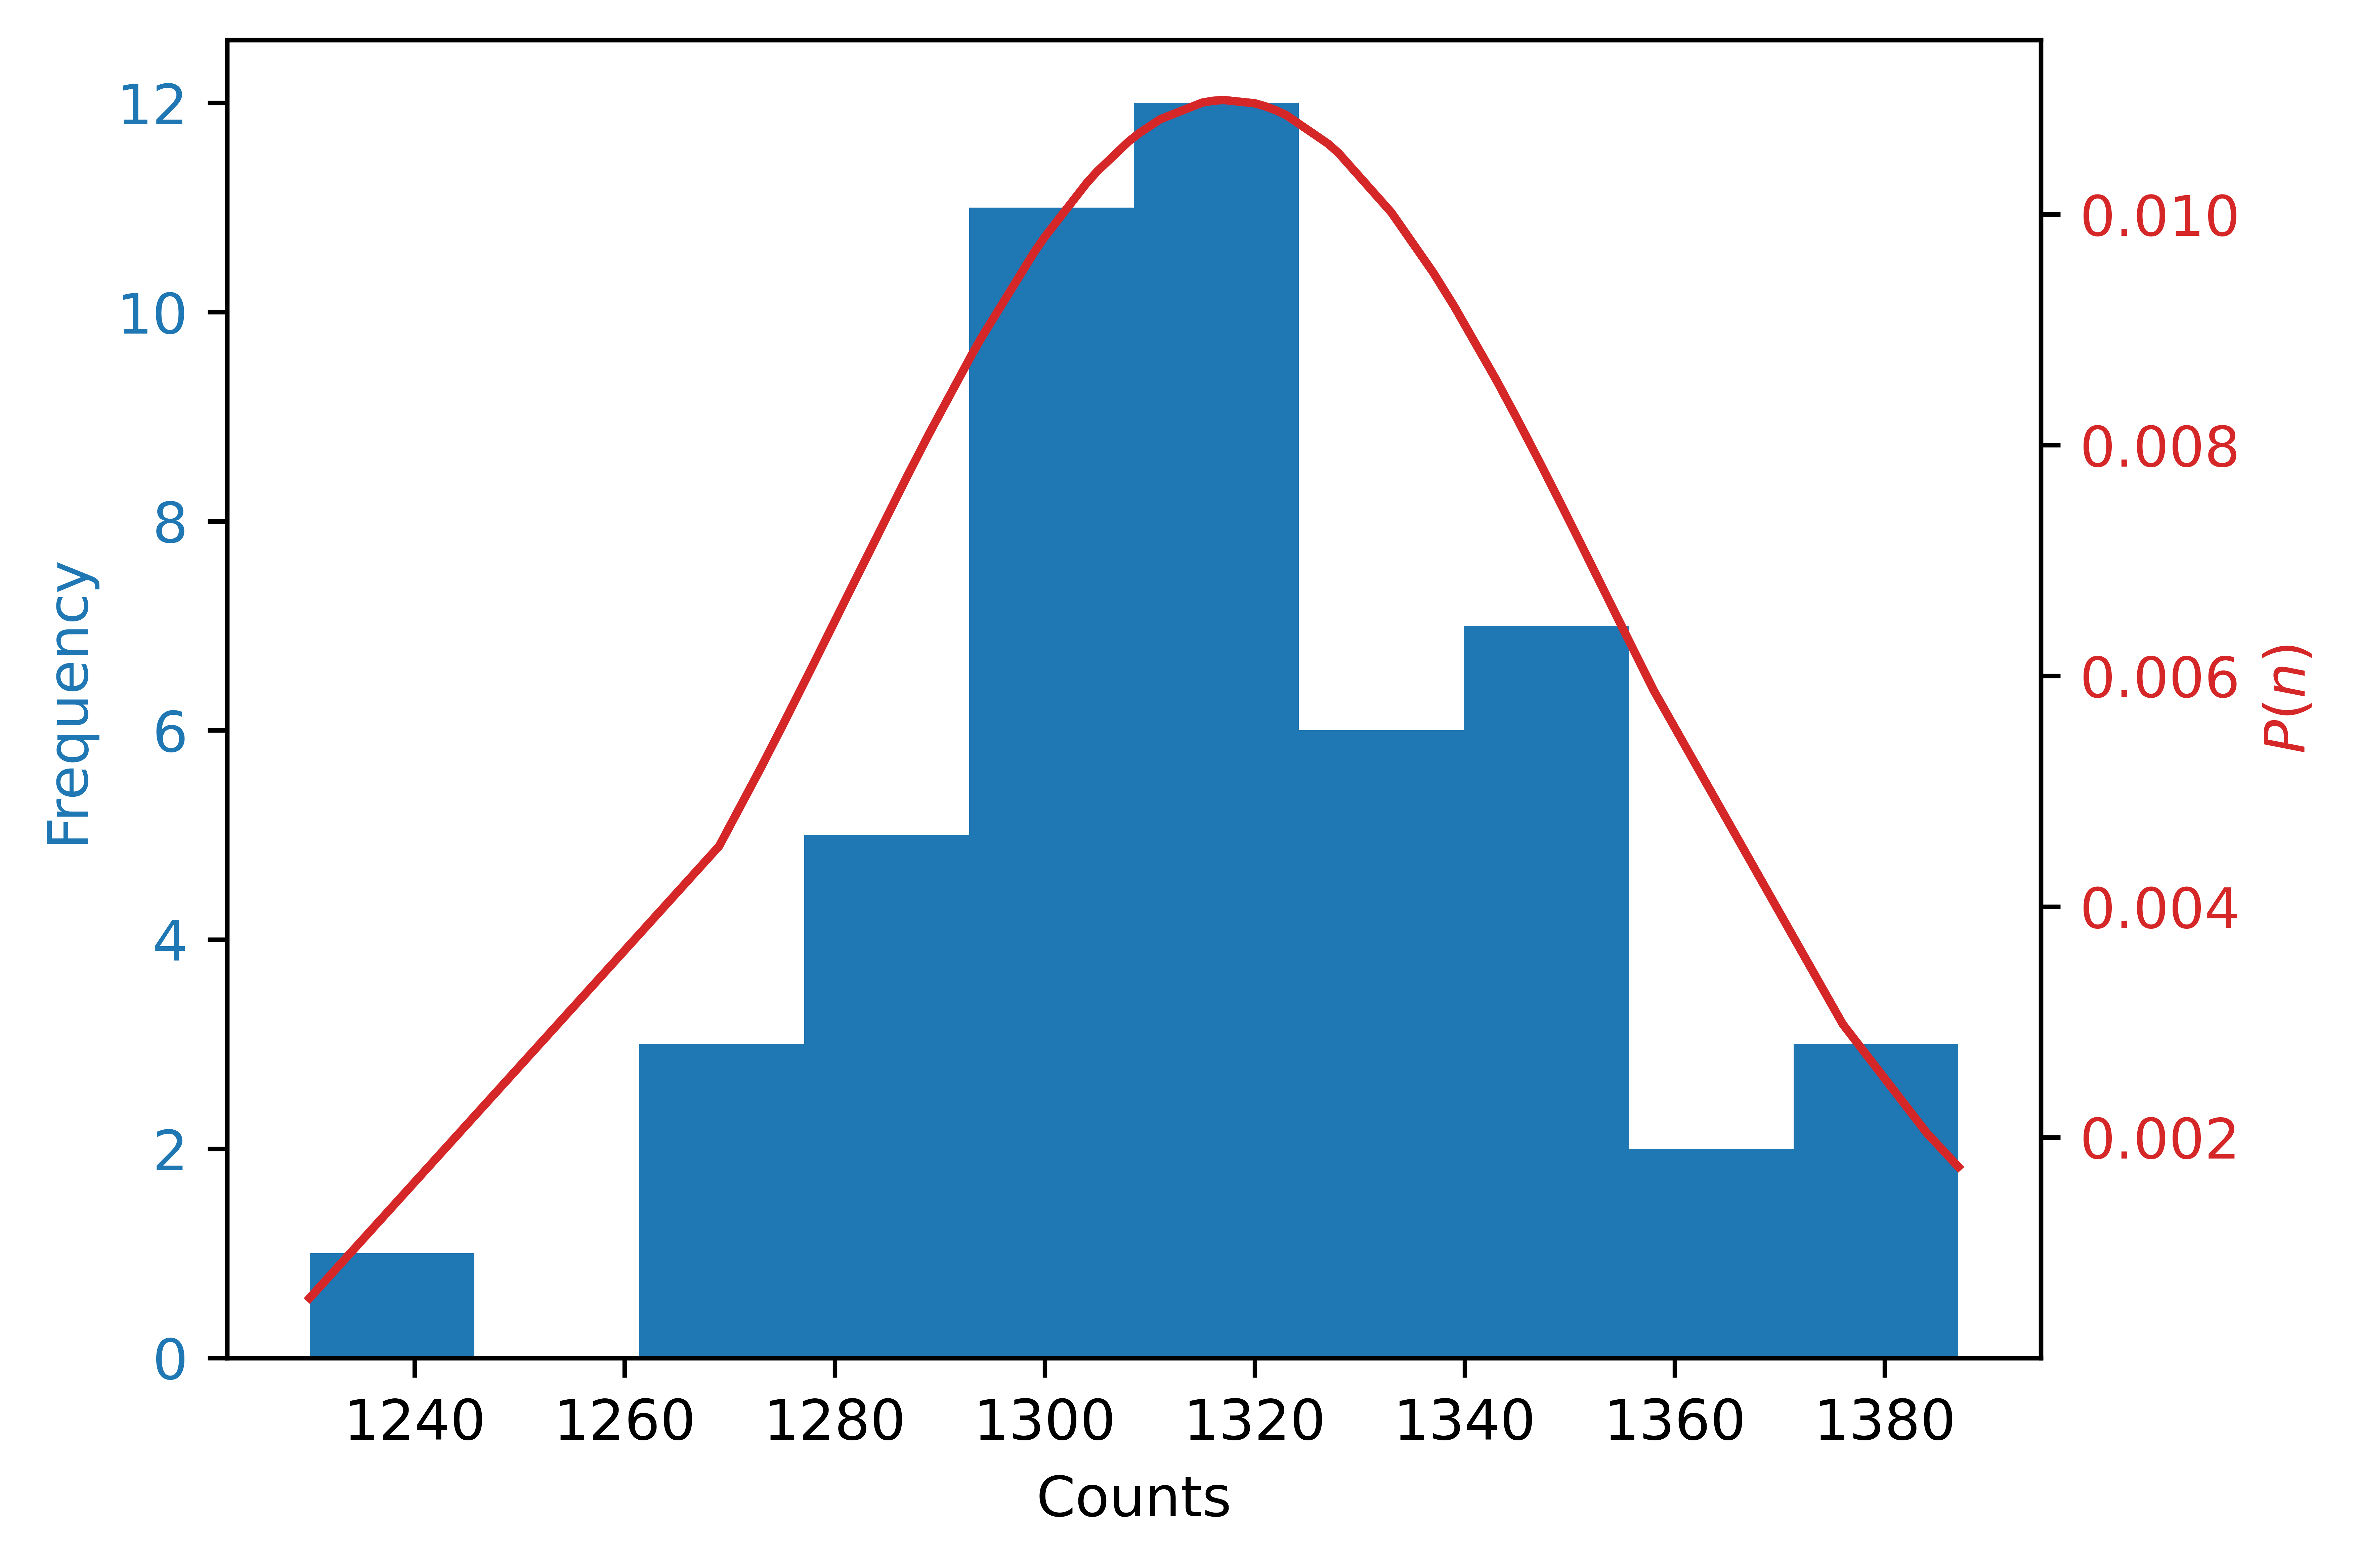
\includegraphics[scale = 0.63]{Figures/plot-ncs-s.png}
            \caption{Histogram for counts with source and overlaid Gaussian curve}
            \label{fig:ncs-s}
        \end{figure}
        \subsubsection{Discussions}
        \begin{enumerate}
            \item The results follow a Poisson distribution on which practically all radioactivity measurements are based. The results show that the mean value N is equal to the variance $\sigma^2$; this is characteristic of the Poisson distribution. The variance in any measured number of counts is therefore equal to the mean value of counts.
            \item The square root of variance, the standard deviation is a measure of the scatter of individual counts around the mean value. As a thumb rule we can say that approximately $2/3$ of the results are within one standard deviation of the mean value i.e., within the interval [($N - \sigma $) and ($N + \sigma$), where $\sigma \sqrt{N}$]. Conversely, given the result from an individual measurement, the unknown \textit{true} count lies within the interval [$N - \sqrt{N}$ and $N + \sqrt{N}$] with a probability of approximately $2/3$.
            \item The above measured results of mean, variance and standard deviation follow Poisson distribution. Results show that the mean value ($N$) is almost equal to the variance ($\sigma^2$) which is characteristic of the Poisson distribution. 
            \item The variance in any measured number of counts is therefore equal to the mean value of counts.
        \end{enumerate}
        \subsubsection{Results}
        \begin{enumerate}
            \item For the background counts, the histogram and Poisson distribution were obtained as expected.
            \item For the counts with source, the histograms and the Gaussian distribution were obtained as expected.
        \end{enumerate}


    \subsection{Efficiency of Geiger-M\"{u}ller Detector}
        By knowing the activity of a gamma source, it is possible to record counts with the source for a known preset time and estimate the efficiency of the G-M detector. We then calculate the efficiency of the detector for a beta source with the only difference being, here we place Beta source about $\SI{2}{\centi \metre}$ close to the end window and calculate \textit{intrinsic efficiency} (which do not take geometry factor into consideration).
        \par
        The equipment required for this experiment are the G-M counting system, the end window detector stand, the G-M detector itself in a cylindrical enclosure, radioactive sources and necessary connecting cables.
        \begin{figure}
            \centering
            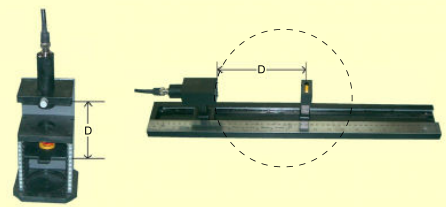
\includegraphics[scale = 0.8]{Figures/gmeff.png}
            \caption{Detector source arrangement for efficiency calculation for a gamma source}
            \label{fig:gmeff}
        \end{figure}
        \begin{table*}[]
        \caption{Reading for determination of efficiency of the G-M counter}
        \label{tab:efficiency}
        \begin{tabular}{@{}cccccccc@{}}
        \toprule
        \multirow{2}{*}{\textbf{\#}} & \multicolumn{3}{c}{\textbf{Gamma source, Cs-137}} & \phantom{a} & \multicolumn{3}{c}{\textbf{Beta source, Tl-204}} \\ \cmidrule{2-4} \cmidrule{6-8} 
         &
          \begin{tabular}[c]{@{}c@{}}\textbf{Background Counts}\\ (100 s)\end{tabular} &
          \begin{tabular}[c]{@{}c@{}}\textbf{Counts}\\ (100 s)\end{tabular} &
          \textbf{Net count rate}, $R_n$ ($s^{-1}$) &&
          \begin{tabular}[c]{@{}c@{}}\textbf{Background   Counts}\\ (100 s)\end{tabular} &
          \begin{tabular}[c]{@{}c@{}}\textbf{Counts} \\ (100 s)\end{tabular} &
          \textbf{Net count rate}, $R_n$ ($s^{-1}$) \\ \midrule
        1                                 & 102    & 854    & 7.52    && 115   & 4011   & 38.96   \\
        2                                 & 109    & 802    & 6.93    && 108   & 3922   & 38.14   \\
        3                                 & 97     & 877    & 7.80    && 110   & 3930   & 38.20   \\
        4                                 & 92     & 842    & 7.50    && 105   & 3890   & 37.85   \\
        5                                 & 110    & 824    & 7.14    && 107   & 3956   & 38.49   \\ \bottomrule
        \end{tabular}
        \end{table*}
        \subsubsection{Data Analysis}
        Gamma source emits radiation isotropically in all directions ($4 \Pi$ geometry). However only fraction of it is received by the end window detector. This fraction is given by
        \begin{equation}
            \dfrac{\Pi d^2/4}{4 \Pi D^2} = \dfrac{d^2}{16 D^2}
        \end{equation}
        where $D$ is the distance from source holder to end window and $d$ is the diameter of end window.
        \par
        The present activity ($A$) of the gamma source used for this experiment is $\SI{75.45}{\kilo \becquerel}$. This gamma source is radiating isotropically in all directions. A fraction of this only is entering the G-M Tube, which is given by
        \begin{equation}
            R = A \times \dfrac{d^2}{16 D^2}
        \end{equation}
        For our experiment, $D = \SI{10}{\centi \metre}$ and $d = \SI{3}{\centi \metre}$. Thus $R = \SI{424.38}{\becquerel}$. Now average net count rate $R$ can be found by calculating the mean of the values for $R$ given in table (\ref{tab:efficiency}). For Cs-137, average count rate is given by $\SI{7.38}{\becquerel}$. Now the efficiency is given by
        \begin{equation}
            E = \dfrac{CPS}{DPS} = \dfrac{R_n}{R}
        \end{equation}
        where $CPS$ is counts per second and $DPS$ is the disintegrations per second falling on the detector window. Thus, efficiency of the G-M counter for gamma source, Cs-137 is
        \begin{equation}
            E = \dfrac{R_n}{R} = \dfrac{7.38}{424.38} = 1.74 \%
        \end{equation}
        Now to calculate the intrinsic efficiency of the beta source, we have average net count rate $R = \SI{38.33}{\becquerel}$. The present activity as calculated earlier is $A = \SI{4120.34}{\kilo \becquerel}$. Thus, efficiency is
        \begin{equation}
            E = \dfrac{CPS}{DPS} = \dfrac{38.33}{4120.34} = 0.93 \%
        \end{equation}
        \subsubsection{Discussions}
        \begin{enumerate}
            \item By knowing the efficiency of the G-M detector for a particular Gamma energy (at a specified distance and geometry), one can further calculate the following parameters, namely activity of the source as on the day of experimentation (of course it is assumed that activity of the standard is known as on the date of manufacture), and also the activity of the unknown source if any with the same energy.
            \item It can be noticed that End Window detector will have much better efficiency for Beta Source compared to a gamma source.
            \item By knowing efficiency for a Beta source , if an unknown activity Beta source is kept for counting one can calculate and find out its activity.
        \end{enumerate}
        \subsubsection{Results}
        \begin{enumerate}
            \item The efficiency of the G-M counter for gamma source was found to be $1.74\%$.
            \item The efficiency of the G-M counter for beta source was found to be $0.93\%$.
        \end{enumerate}


    \subsection{Feather Analysis}
        The purpose of Feather analysis is to carry out the absorption studies on $\beta$-rays with the aid of a G-M Counter and hence to determine the end point energy of $\beta$-rays emitted from a radioactive source.
        \par
        The equipment required for this experiment are the G-M counting system, the end window detector stand, the G-M detector itself, beta source and Aluminium absorber kit.
        \begin{table}[]
        \caption{Readings for Feather Analysis experiment for Tl-204}
        \label{tab:feathertl204}
        \setlength{\tabcolsep}{10pt}
        \begin{tabular}{@{}cccc@{}}
        \toprule
          \begin{tabular}[c]{@{}c@{}}\textbf{Absorber} \\ \textbf{Thickness}\\  (mm)\end{tabular} &
          \begin{tabular}[c]{@{}c@{}}\textbf{Absorber}   \\ \textbf{Thickness} \\ (mg $cm^{-2}$)\end{tabular} &
          \begin{tabular}[c]{@{}c@{}}\textbf{Counts}\\ (180 s)\end{tabular} &
          \textbf{Net Counts} \\ \midrule
        0    & 0     & 7412 & 7217 \\
        0.06 & 16.26 & 5403 & 5208 \\
        0.12 & 32.52 & 4132 & 3937 \\
        0.18 & 48.78 & 3196 & 3001 \\
        0.24 & 65.04 & 1893 & 1698 \\
        0.3  & 81.3  & 1897 & 1702 \\
        0.36 & 97.56 & 1521 & 1326 \\ \bottomrule
        \end{tabular}
        \end{table}
        \begin{table}[]
        \caption{Readings for Feather Analysis experiment for Sr-90}
        \label{tab:feathersr90}
        \setlength{\tabcolsep}{10pt}
        \begin{tabular}{@{}cccc@{}}
        \toprule
          \begin{tabular}[c]{@{}c@{}}\textbf{Absorber}  \\ \textbf{Thickness}\\  (mm)\end{tabular} &
          \begin{tabular}[c]{@{}c@{}}\textbf{Absorber}   \\ \textbf{Thickness} \\ (mg $cm^{-2}$)\end{tabular} &
          \begin{tabular}[c]{@{}c@{}}\textbf{Counts} \\ (100 s)\end{tabular} &
          \textbf{Net counts} \\ \midrule
        0    & 0     & 4781 & 4673 \\
        0.06 & 16.26 & 4335 & 4227 \\
        0.12 & 32.52 & 4120 & 4012 \\
        0.18 & 48.78 & 3737 & 3629 \\
        0.24 & 65.04 & 3689 & 3581 \\
        0.3  & 81.3  & 3610 & 3502 \\
        0.36 & 97.56 & 3233 & 3125 \\
        0.42 & 113.8 & 3134 & 3026 \\
        0.48 & 130.1 & 3323 & 3215 \\
        0.54 & 146.3 & 2900 & 2792 \\
        0.66 & 178.9 & 2618 & 2510 \\
        0.72 & 195.1 & 2405 & 2297 \\
        0.78 & 211.4 & 2252 & 2144 \\
        0.9  & 243.9 & 2021 & 1913 \\
        1.02 & 276.4 & 1781 & 1673 \\ \bottomrule
        \end{tabular}
        \end{table}
        \begin{figure}
            \centering
            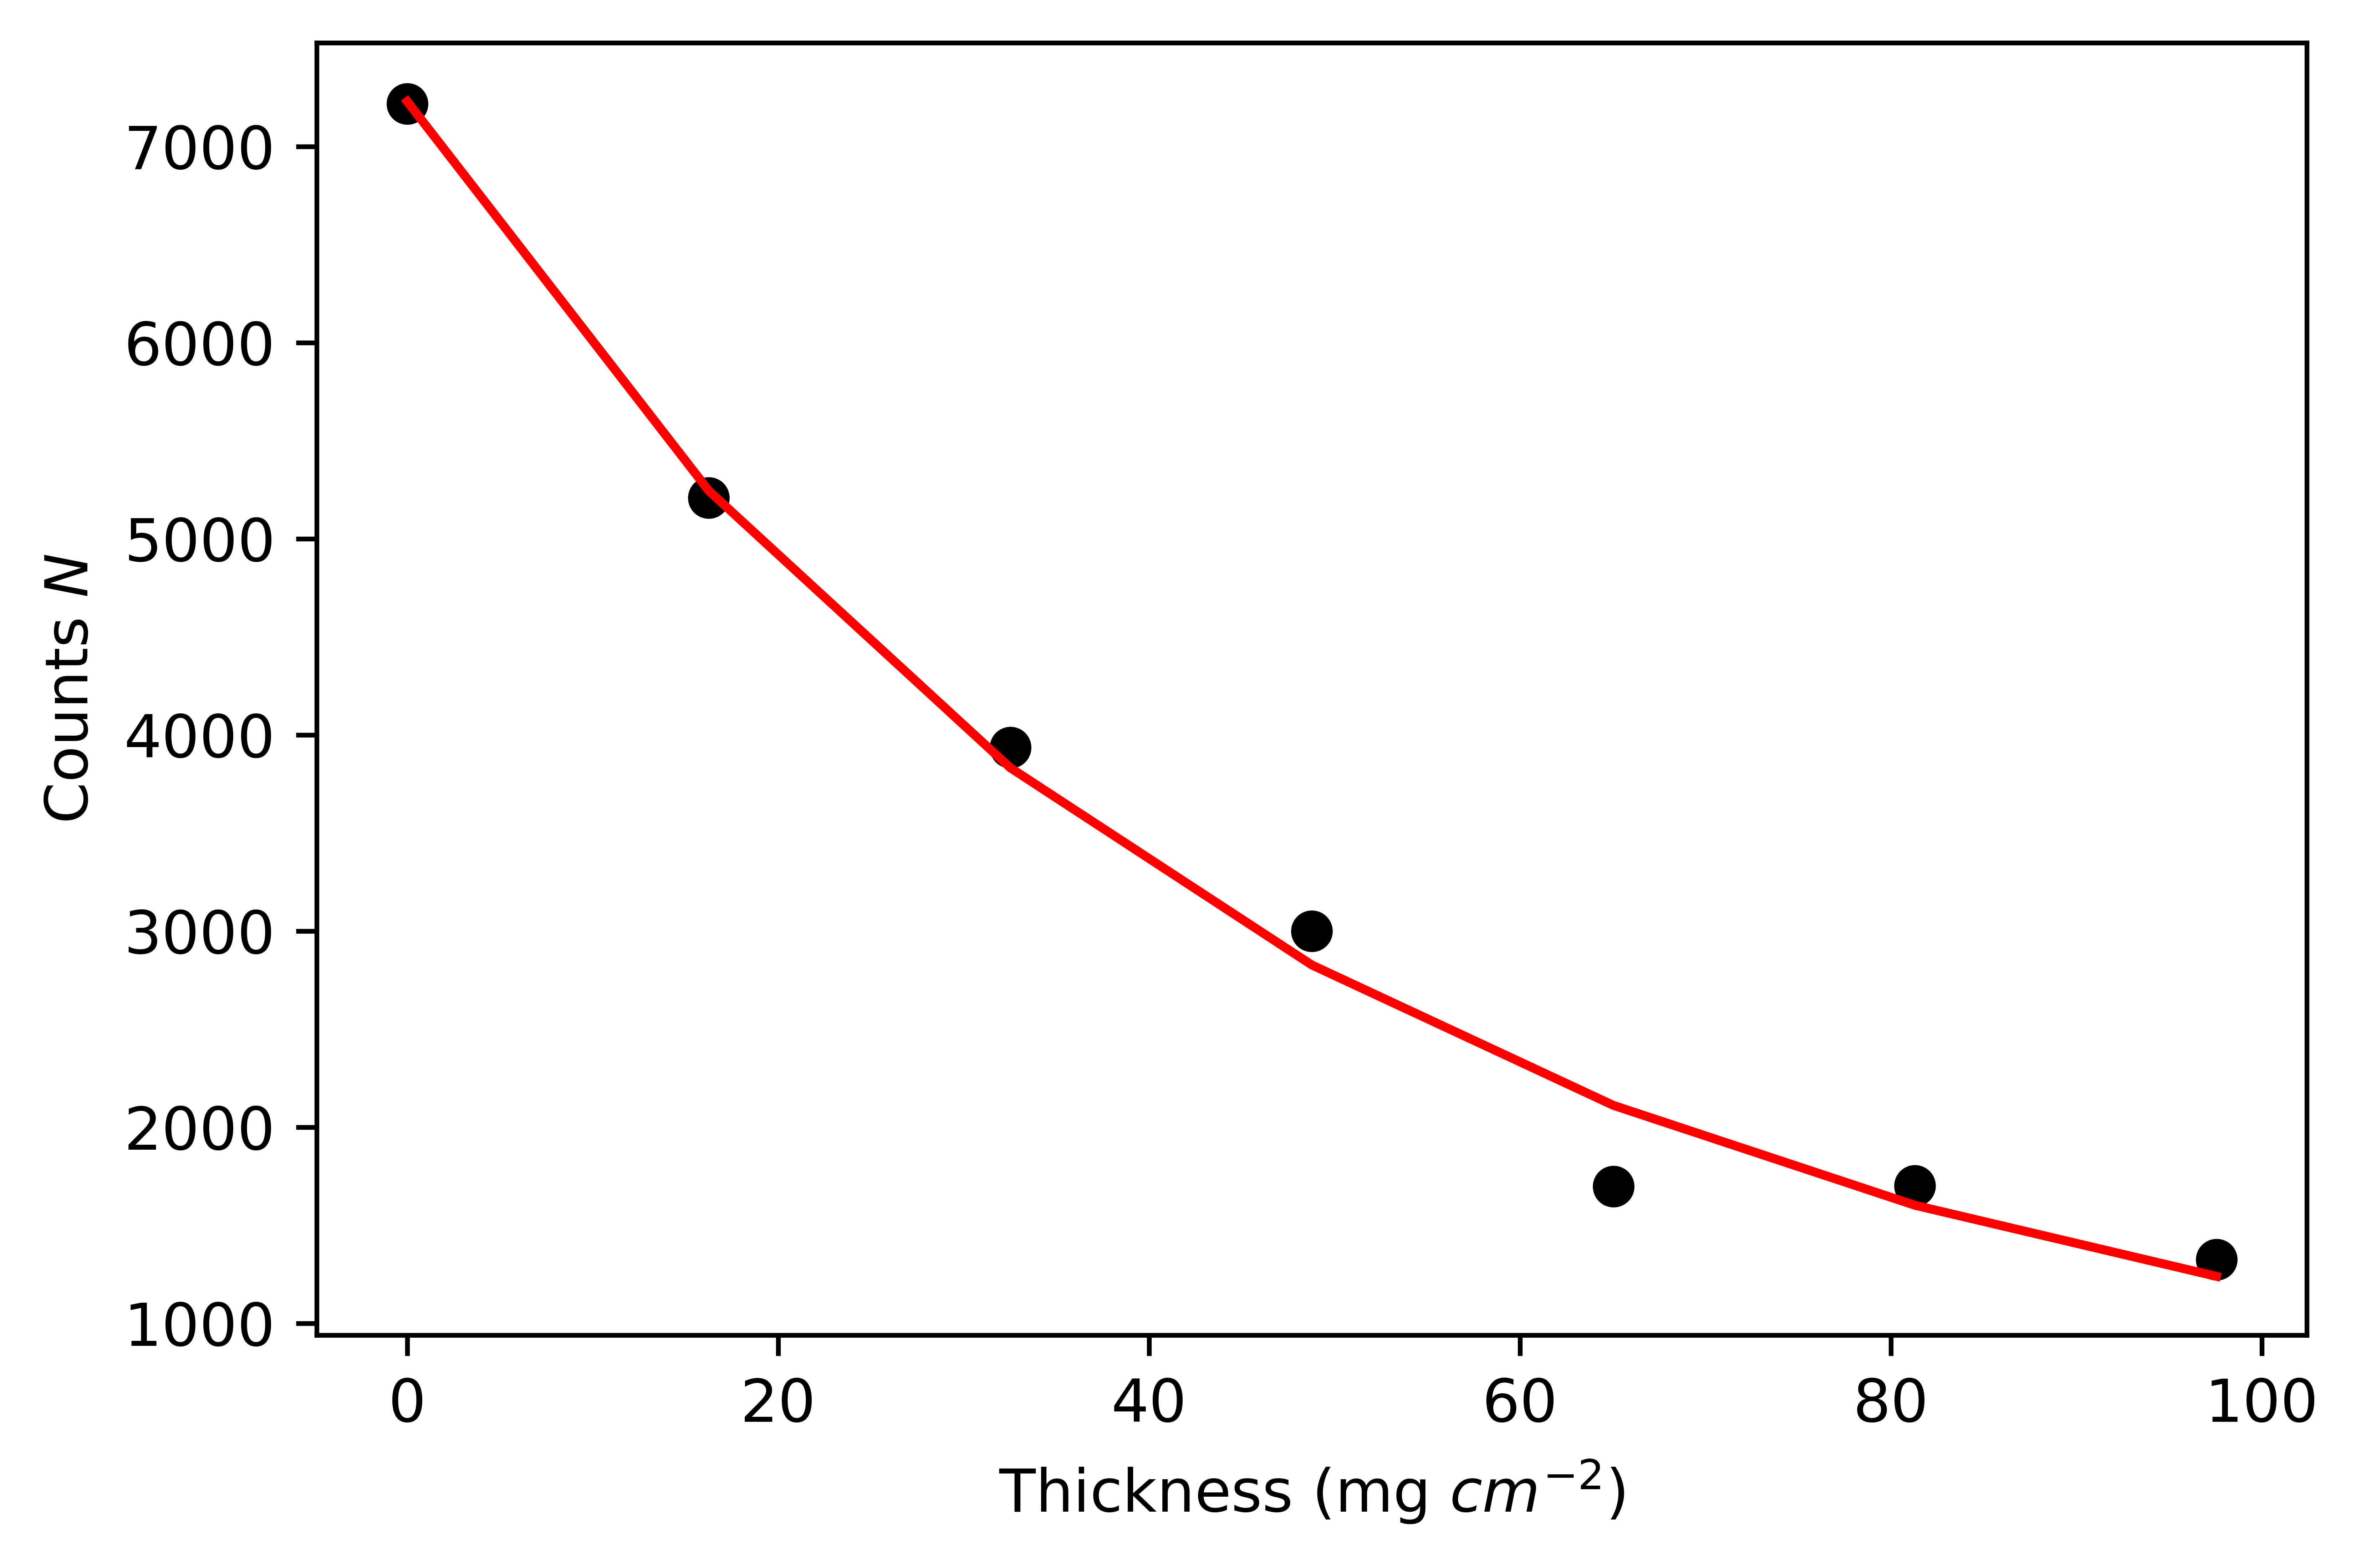
\includegraphics[scale = 0.63]{Figures/plot-feather-1.png}
            \caption{Feather analysis plot for Tl-204}
            \label{fig:feather-1}
        \end{figure}
        \begin{figure}
            \centering
            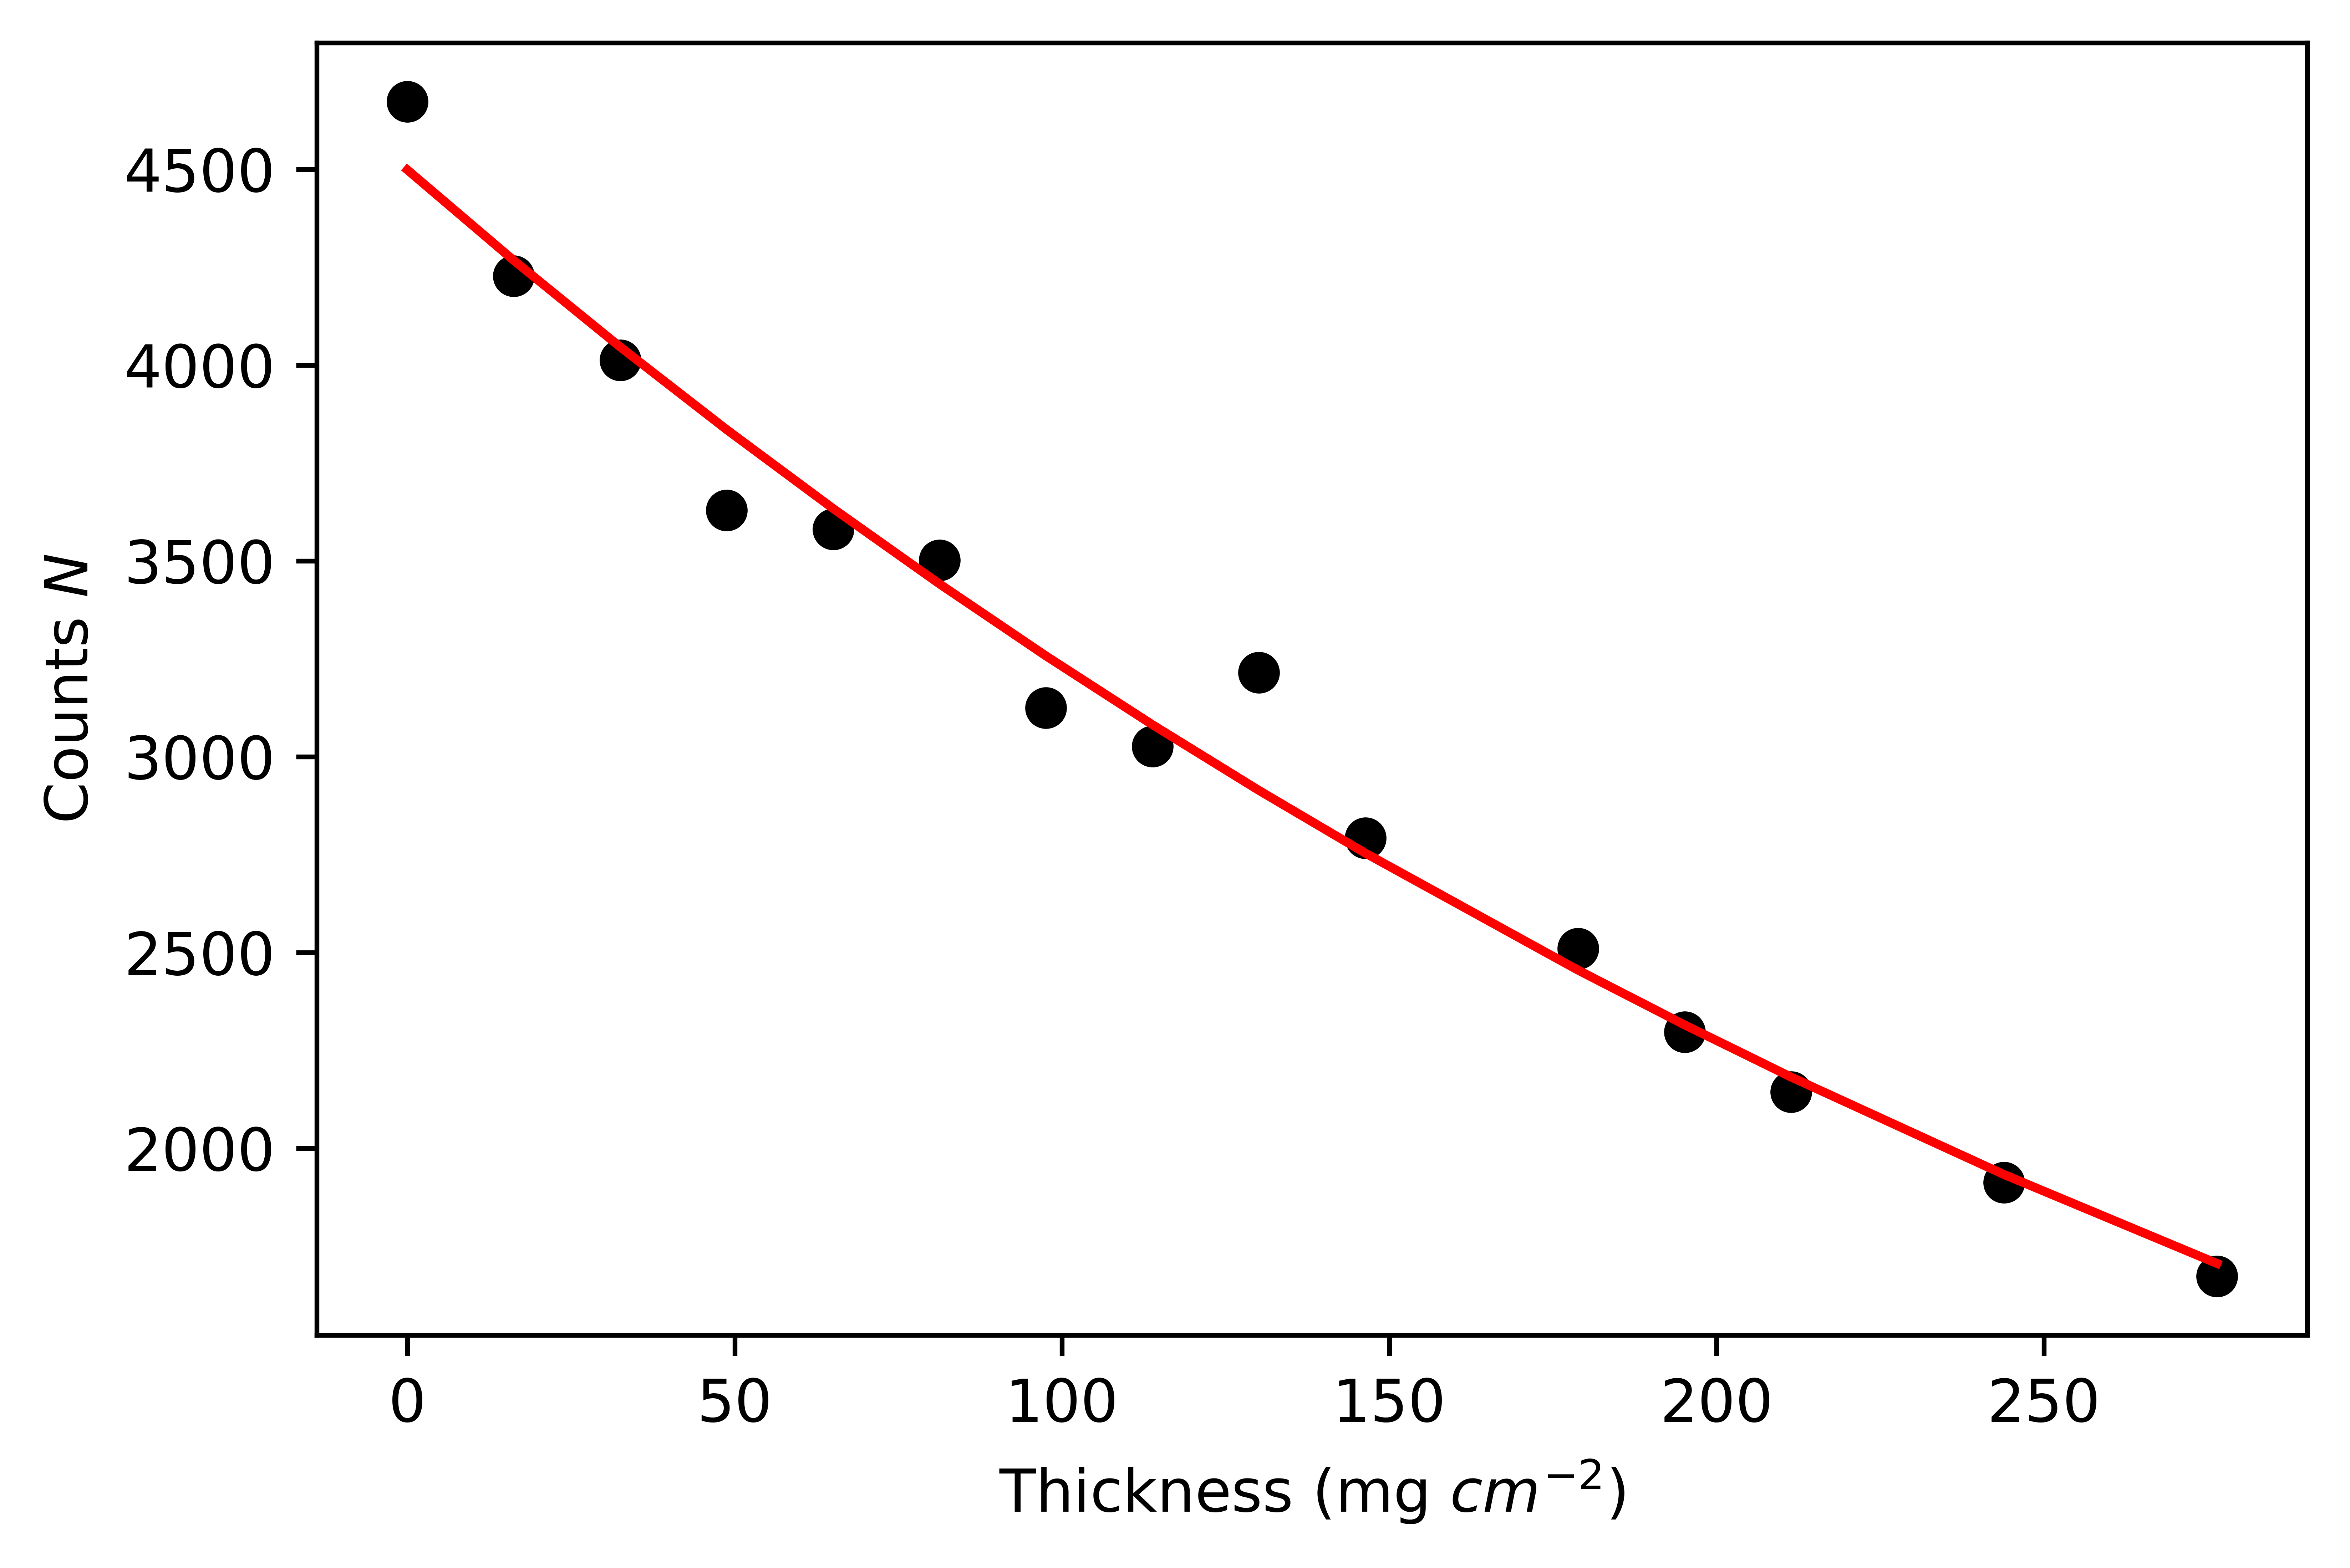
\includegraphics[scale = 0.63]{Figures/plot-feather-2.png}
            \caption{Feather analysis plot for Sr-90}
            \label{fig:feather-2}
        \end{figure}
        \subsubsection{Data Analysis}
        The range of beta particles is given by
        \begin{equation}
            R_0 = (0.52 E_0 - 0.09) \si{\gram \per \centi \metre \squared}
        \end{equation}
        Where $E_0$ is the end point energy of of Beta rays from the radioactive source in $\si{\mega \electronvolt}$.
        \par
        We have the ratio of thickness required to reduce the counts of Beta rays from one source to half to the thickness required for the other source is given by
        \begin{equation}
            \dfrac{t_1 \sfrac{1}{2}}{t_2 \sfrac{1}{2}} = \dfrac{\text{Range of Beta rays from first source}}{\text{Range of Beta rays from second source}}
        \end{equation}
        That is
        \begin{equation}
            \dfrac{t_1 \sfrac{1}{2}}{t_2 \sfrac{1}{2}} = \dfrac{R_1}{R_2}
        \end{equation}
        Now, end point energy of Tl-204 is $\SI{0.764}{\mega \electronvolt}$. Therefore the range of Tl-204, $R_1 = \SI{0.30728}{\gram \per \centi \metre \squared}$. From the figure (\ref{fig:feather-1}), thickness of Al absorber required to reduce the count rate of Tl-204 by half, $t_1 \sfrac{1}{2} = \SI{35.7}{\milli \gram \per \centi \metre \squared}$. From the figure (\ref{fig:feather-2}), thickness of Al absorber required to reduce the count rate of Sr-90 by half, $t_2 \sfrac{1}{2} = \SI{59.4}{\milli \gram \per \centi \metre \squared}$. Therefore, we have
        \begin{equation}
            R_2 = R_1 \times \dfrac{t_2 \sfrac{1}{2}}{t_1 \sfrac{1}{2}} = \SI{0.511}{\gram \per \centi \metre \squared}
        \end{equation}
        Thus, end point energy of Sr-90 is
        \begin{equation}
            E_2 = \dfrac{R_2 +0.09}{0.52} = \SI{1.16}{\mega \electronvolt}
        \end{equation}
        \subsubsection{Results}
        The end point energy of $\beta$-rays from Sr-90 was obtained to be $\SI{1.16}{\mega \electronvolt}$.



    \subsection{Backscattering of Beta Particles}
        When Beta Particles collide with matter, absorption may occur. Another possible result is the occurrence of scattering by collisions of Beta particles with electrons in the material. Such a collision changes the speed and direction of the Beta particles. With increasing atomic number $Z$ of the material, the chance that a collision results in a scattering of the Beta particle increases too. Back scattering occurs, when the angle of deflection is greater than $90 \degree$. The Back-scattering rate is predominately dependent on the atomic number $Z$ of the back scattering material. With an atom of high atomic number, the scattering occurs at a large angle and with little loss of energy. The back scattering factor is approximately proportional to the square root of atomic number. The mass per unit area (thickness $\times$ density) or the thickness of the irradiated material only influence the back scattering factor up to a saturation value. The maximum back scattering is practically attained at a mass per unit area which is smaller than half the range of the Beta particle in the material, because large layer thicknesses lead to absorption of the scattered electrons. The saturation value is less than $\SI{200}{\milli \gram \per \centi \metre \squared}$ for all materials. This corresponds to a saturation larger thickness of $x < \SI{0.74}{\milli \metre}$ for Aluminum and $x < \SI{0.17}{\milli \metre}$ for Lead.
        \begin{figure}
            \centering
            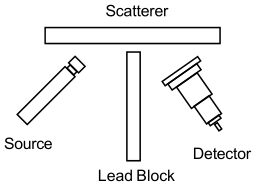
\includegraphics{Figures/bacscattSCHEMATIC.png}
            \caption{Schematic diagram for Backscattering experiment}
            \label{fig:bacscattschematic}
        \end{figure}
        \par
        The equipment required for this experiment are the electronic unit, the wide end window G-M detector, the absorber stand for Back scattering of Beta, absorber set, beta source and Lead block for isolation.
        \begin{figure}
            \centering
            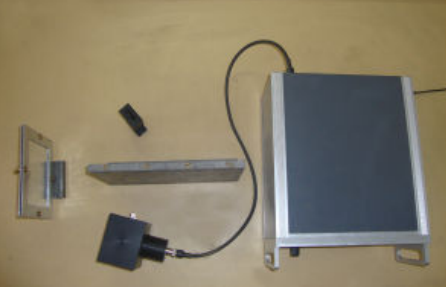
\includegraphics[scale = 0.8]{Figures/backscattTOP.png}
            \caption{Experimental set-up for Backscattering experiment}
            \label{fig:backscattTOP}
        \end{figure}
        \begin{figure}
            \centering
            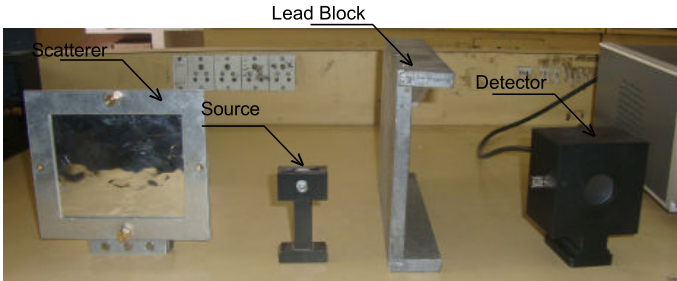
\includegraphics[scale = 0.6]{Figures/backscattSIDE.png}
            \caption{Individual blocks of experiment setup}
            \label{fig:backscattSIDE}
        \end{figure}
        \begin{table}[]
        \caption{Reading for Backscattering of Beta particles experiment}
        \label{tab:backscatter}
        \setlength{\tabcolsep}{18pt}
        \begin{tabular}{@{}ccc@{}}
        \toprule
        \begin{tabular}[c]{@{}c@{}}\textbf{Thickness}  \\ \textbf{of Al foil} \\ (mm)\end{tabular} & \begin{tabular}[c]{@{}c@{}}\textbf{Counts}\\ (200 s) \end{tabular} & \textbf{Net Counts} \\ \midrule
        0    & 344 & 0   \\
        0.05 & 587 & 243 \\
        0.1  & 662 & 318 \\
        0.15 & 683 & 339 \\
        0.2  & 767 & 423 \\
        0.25 & 814 & 470 \\
        0.3  & 843 & 499 \\
        0.35 & 878 & 534 \\
        0.4  & 824 & 480 \\
        0.45 & 795 & 451 \\ \bottomrule
        \end{tabular}
        \end{table}

        \subsubsection{Results}
        From the obtained results, it can be concluded that the counts due to Back scattering increases up to certain thickness of the scattering material and almost remains constant beyond that thickness. The thickness of the scatterer, where the counts reach their maximum is called the Saturation thickness.


    \subsection{Production and Attenuation of Bremsstrahlung}
        Bremsstrahlung is electromagnetic radiation produced by the deceleration of a charged particle when deflected by another charged particle, typically an electron by an atomic nucleus. The moving particle loses kinetic energy, which is converted into a photon because energy is conserved. The term is also used to refer to the process of producing the radiation. Bremsstrahlung has a continuous spectrum which becomes more intense and whose intensity shifts toward higher frequencies as the change of the energy of the accelerated particles increases.
        \par
        Beta – particle emitting substances sometimes exhibit a weak radiation with continuous spectrum that is due to Bremsstrahlung. In this context, Bremsstrahlung is a type of \textit{secondary radiation}, in that it is produced as a result of stopping (or slowing) the primary radiation (Beta particles). It is very similar to x-rays produced by bombarding metal targets with electrons in X-ray machines.
        \par
        The amount of Bremsstrahlung increases as the atomic number/density of the absorbing material goes up. If the mass per unit area (thickness X density) of the plates used as absorbers is such that the beta particles are completely absorbed, then for materials of higher atomic number/density, correspondingly higher Bremsstrahlung count rates are obtained.
        \par
        The equipment required for this experiment are the electronic unit, the G-M detector, detector holder, sliding bench, source holder, absorber Holder, beta source and Al (\SI{0.7}{\milli \metre}), Cu (\SI{0.3}{\milli \metre}) and Perspex (\SI{1.8}{\milli \metre}).
        \begin{figure}
            \centering
            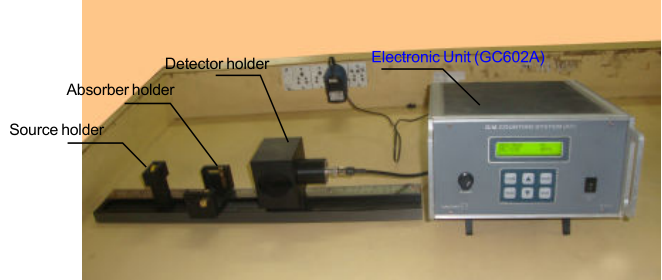
\includegraphics[scale = 0.6]{Figures/brem.png}
            \caption{Experimental set-up for the Bremsstrahlung experiment}
            \label{fig:brem}
        \end{figure}
        \begin{table}[]
            \caption{Readings for Bremsstrahlung experiment}
            \label{tab:brem}
            \begin{subtable}[h]{0.45\textwidth}
                \centering
                \caption{For Al (0.7mm) and Perspex (1.8mm) combination:}
                \label{tab:alperspex}
                \setlength{\tabcolsep}{2.5pt}
                \begin{tabular}{@{}clcc@{}}
                \toprule
                \textbf{\#} & \textbf{Position} & \begin{tabular}[c]{@{}c@{}}\textbf{Counts}\\ (300 s)\end{tabular} & \textbf{Net Counts} \\ \midrule
                1 & \textit{Aluminium facing   source} & 798  & 546  \\
                2 & \textit{Perspex facing source}     & 792  & 540  \\
                3 & \textit{No Absorber}               & 8342 & 8090 \\ \bottomrule
                \end{tabular}
            \end{subtable}
            \hfill
            \begin{subtable}[h]{0.45\textwidth}
                \centering
                \caption{For Perspex (1.8mm) and Cu (0.3mm) combination:}
                \label{tab:cuperspex}
                \setlength{\tabcolsep}{5pt}
                \begin{tabular}{@{}clcc@{}}
                \toprule
                \textbf{\#} & \textbf{Position} & \begin{tabular}[c]{@{}c@{}}\textbf{Counts}\\ (300 s)\end{tabular} & \textbf{Net Counts} \\ \midrule
                1 & \textit{Perspex facing source} & 498  & 246  \\
                2 & \textit{Copper facing source}  & 535  & 283  \\
                3 & \textit{No Absorber}           & 8556 & 8304 \\ \bottomrule
                \end{tabular}
            \end{subtable}
            \hfill
            \begin{subtable}[h]{0.45\textwidth}
                \centering
                \caption{For Al (1.8mm) and Cu (0.3mm) combination:}
                \label{tab:alcu}
                \setlength{\tabcolsep}{2.5pt}
                \begin{tabular}{@{}clcc@{}}
                \toprule
                \textbf{\#} & \textbf{Position} & \begin{tabular}[c]{@{}c@{}}\textbf{Counts}\\ (300 s)\end{tabular} & \textbf{Net Counts} \\ \midrule
                1 & \textit{Aluminium facing   source} & 523  & 271  \\
                2 & \textit{Copper facing source}      & 542  & 290  \\
                3 & \textit{No Absorber }              & 8259 & 8007 \\ \bottomrule
                \end{tabular}
            \end{subtable}
        \end{table}
        \subsubsection{Discussions}
        \begin{enumerate}
            \item The count rate for the Bremsstrahlung produced depends on the order in which the absorbent materials are arranged. If, firstly, the sheet of metal faces towards the source, then a higher count rate is measured since Bremsstrahlung is generated in the aluminium but is absorbed to a very small extent in the sheet of Perspex which follows.
            \item If, however, the beta rays first strike the sheet of plastic, then the Bremsstrahlung generated is of low energy and a large proportion of it is absorbed in the sheet of metal which follows. These conclusions can be extended to other combinations of materials also.
        \end{enumerate}
        \subsubsection{Results}


    \subsection{Measurement of Short Half-life}
        The purpose of this experiment is to determine short half-life of a given source, which can be obtained from a mini generator or produced with a neutron source by activation. The equipment required for this experiment are the G-M counting system, the end window detector stand, the G-M detector itself and a short half-life source.
        \begin{table*}[]
        \caption{Readings for short half-life experiment}
        \label{tab:half-life}
        \setlength{\tabcolsep}{15pt}
        \begin{tabular}{@{}ccccc@{}}
        \toprule
        \textbf{Elapsed   Time} (s) & \textbf{Counts} & \textbf{Corrected counts} & \textbf{Corrected counts}, $N$ ($s^{-1}$) & $\ln N$  \\ \midrule
        10               & 2001   & 1988             & 199                      & 5.292 \\
        20               & 3892   & 3866             & 193                      & 5.264 \\
        30               & 5663   & 5624             & 187                      & 5.234 \\
        40               & 7377   & 7325             & 183                      & 5.21  \\
        50               & 8961   & 8896             & 178                      & 5.181 \\
        60               & 10535  & 10457            & 174                      & 5.161 \\
        70               & 12057  & 11966            & 171                      & 5.141 \\
        80               & 13447  & 13343            & 167                      & 5.117 \\
        90               & 14751  & 14634            & 163                      & 5.091 \\
        100              & 16045  & 15915            & 159                      & 5.07  \\
        110              & 17256  & 17113            & 156                      & 5.047 \\
        120              & 18416  & 18260            & 152                      & 5.025 \\
        130              & 19498  & 19329            & 149                      & 5.002 \\
        140              & 20514  & 20332            & 145                      & 4.978 \\
        150              & 21470  & 21275            & 142                      & 4.955 \\
        160              & 22380  & 22172            & 139                      & 4.931 \\
        170              & 23268  & 23047            & 136                      & 4.909 \\
        180              & 24051  & 23817            & 132                      & 4.885 \\
        190              & 24841  & 24594            & 129                      & 4.863 \\
        200              & 25577  & 25317            & 127                      & 4.841 \\
        210              & 26286  & 26013            & 124                      & 4.819 \\
        220              & 26942  & 26656            & 121                      & 4.797 \\
        230              & 27578  & 27279            & 119                      & 4.776 \\
        240              & 28221  & 27909            & 116                      & 4.756 \\
        250              & 28796  & 28471            & 114                      & 4.735 \\
        260              & 29345  & 29007            & 112                      & 4.715 \\
        270              & 29911  & 29560            & 109                      & 4.696 \\
        280              & 30428  & 30064            & 107                      & 4.676 \\
        290              & 30925  & 30548            & 105                      & 4.657 \\
        300              & 31365  & 30975            & 103                      & 4.637 \\ \bottomrule
        \end{tabular}
        \end{table*}
        \begin{figure}
            \centering
            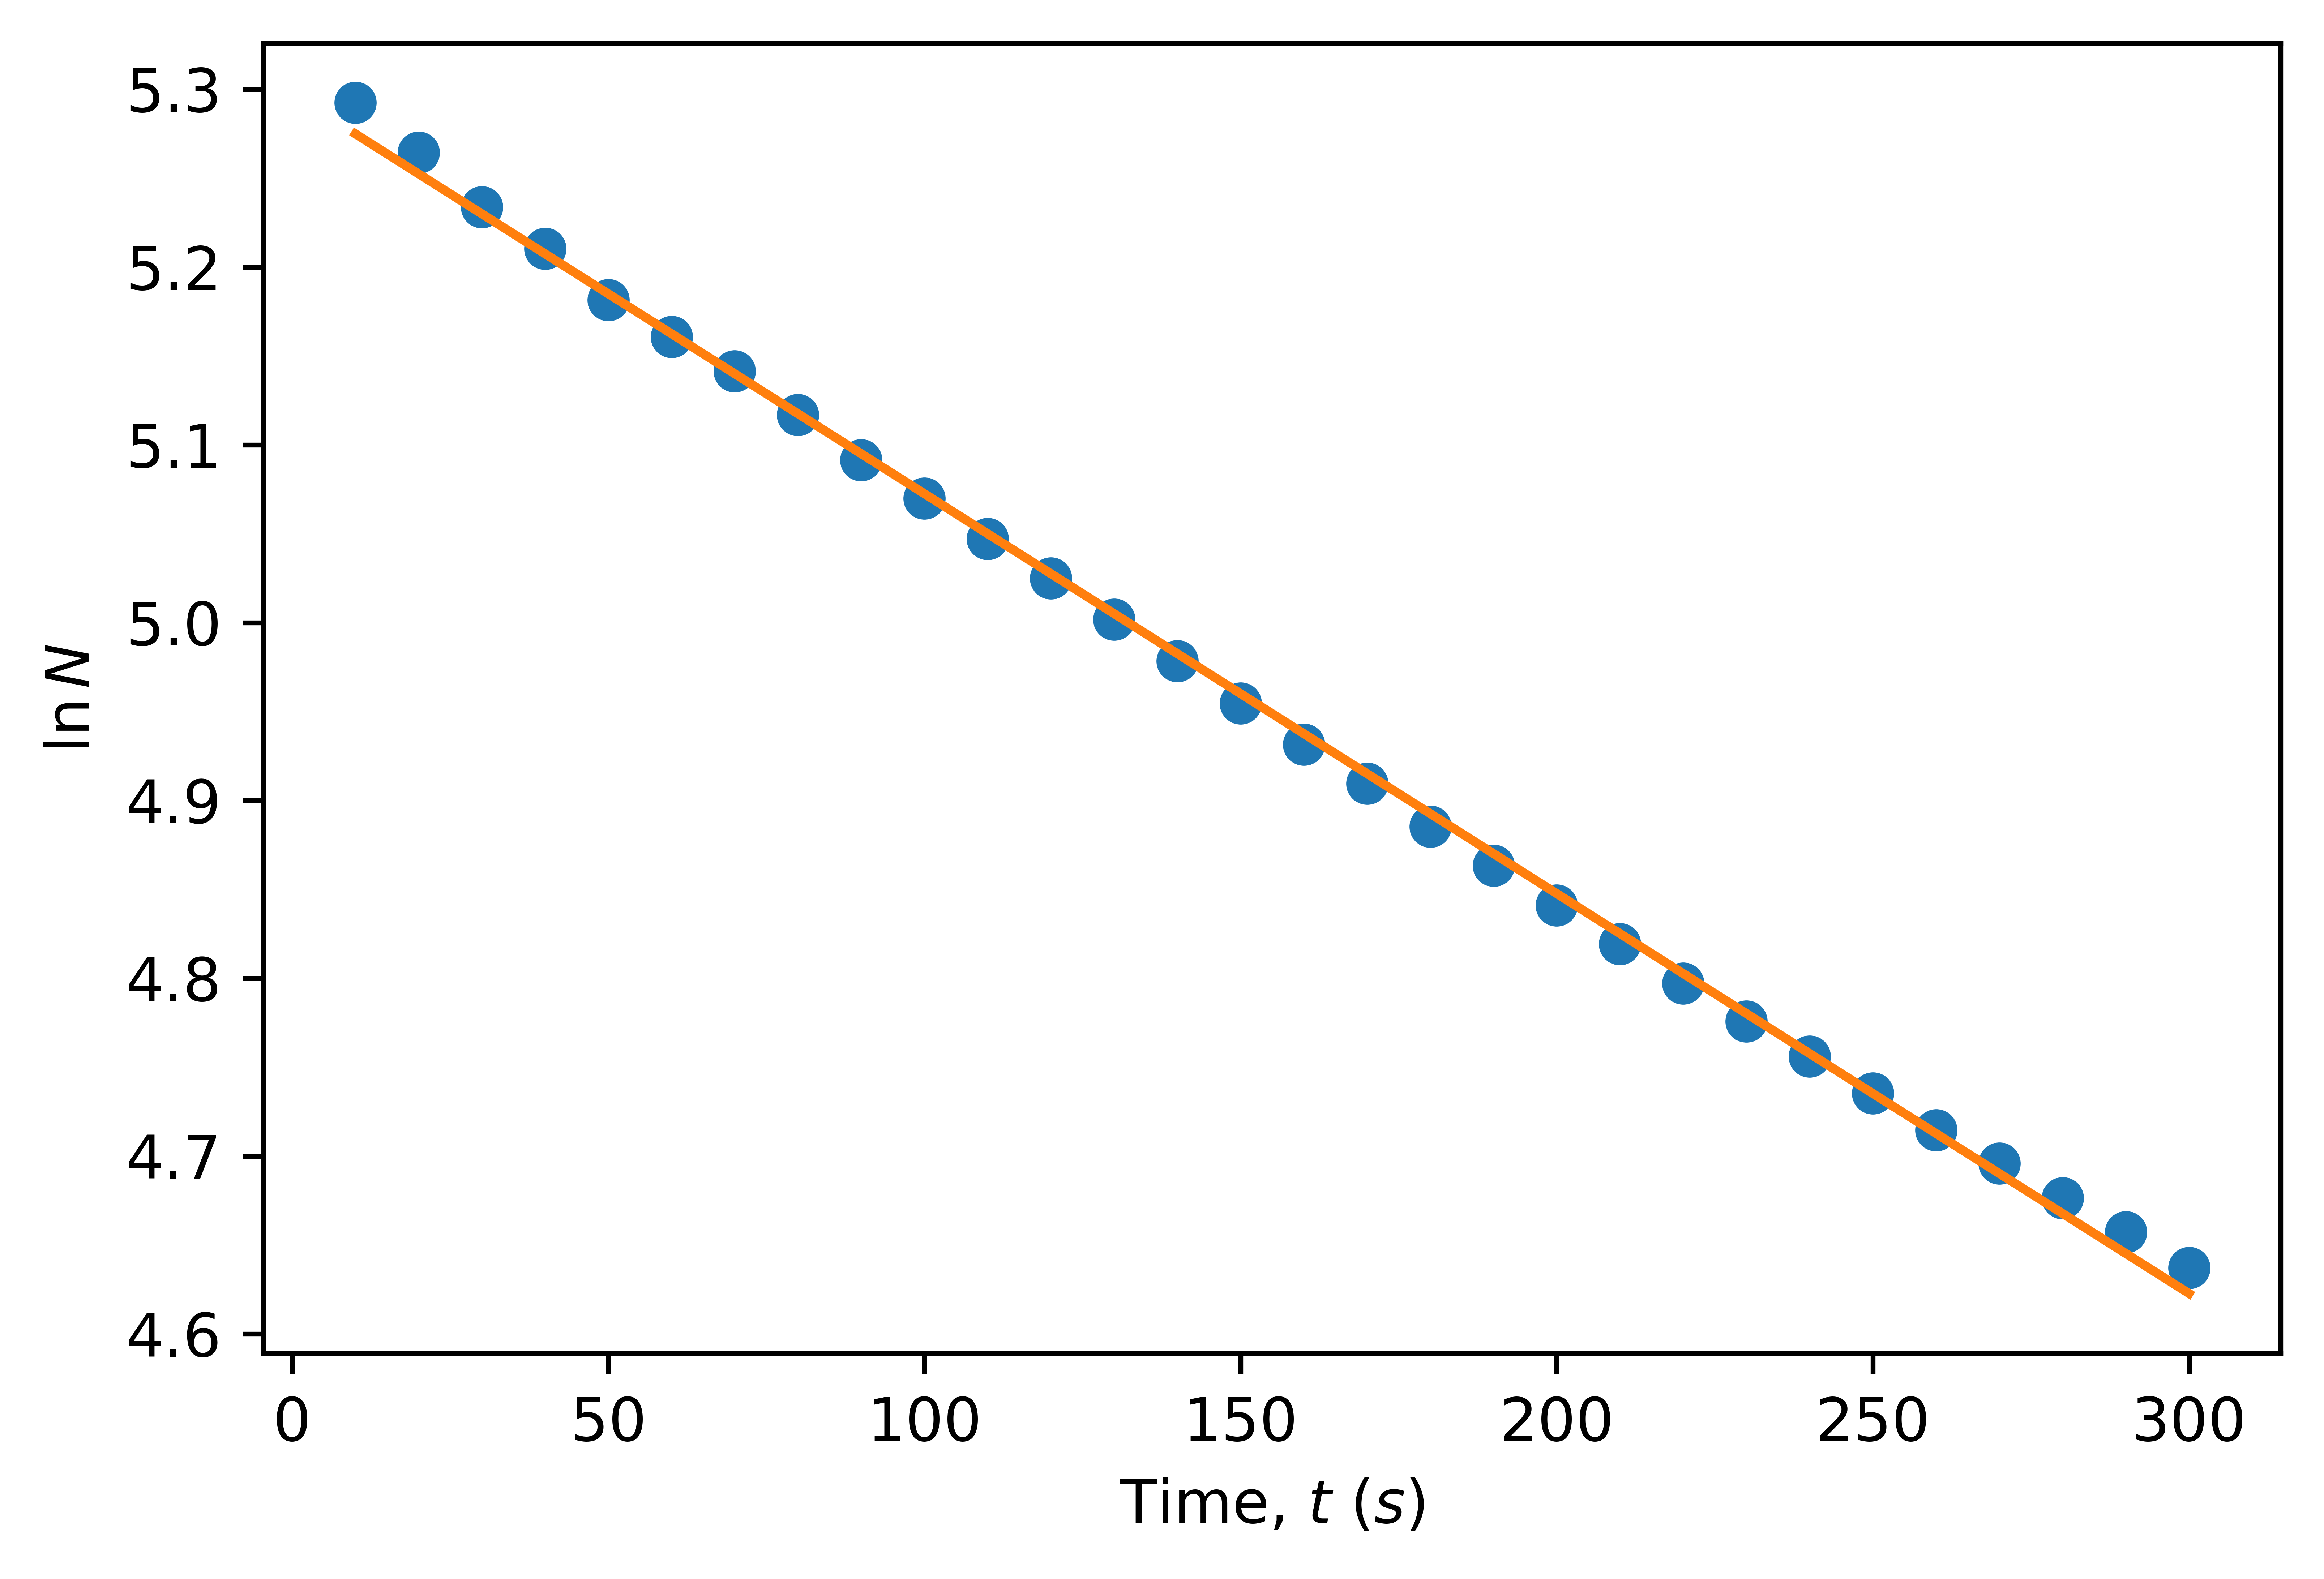
\includegraphics[scale = 0.63]{Figures/plot-half-life.png}
            \caption{Plot between $\log S$ and time, $t$ for half-life experiment}
            \label{fig:half-life}
        \end{figure}
        \subsubsection{Calculations}
        Intensity of radioactive source changes with time in accordance with relation
        \begin{equation}
            I = I_0 e^{-\lambda t}
        \end{equation}
        where $\lambda$ is the decay constant, $I$ is the intensity at any time $t$ and $I_0$ is the initial intensity. The $T_{1/2}$ by definition is the time required for the intensity to fall to one half of its initial value. Hence, we have
        \begin{equation}
            \begin{split}
                \ln (I/I_0) = -\lambda T_{1/2} \\
                \ln(0.5) = -\lambda T_{1/2} \\
                \dfrac{0.693}{\lambda} = T_{1/2} \\
                \implies \lambda = \dfrac{0.693}{T_{1/2}}
            \end{split}
        \end{equation}
        Using the data from table (\ref{tab:half-life}), we plot the figure (\ref{fig:half-life}). From here we calculate the slope using least square fit as
        \begin{equation}
        \label{slope}
            m = \dfrac{S S_{xy} - S_{x}S_{y}}{S S_{xx} - S_{x}^2}
        \end{equation}
        where $S$ is the number of observations, $x$ is the time interval and $y$ is $\ln S$. Putting in the values, we get slope, $m = \SI{-224.88e-5}{\per \second}$. This slope should be equal to the negative of the decay constant $\lambda$ as is evident from our formula. Therefore $\lambda = \SI{224.88e-5}{\per \second}$. And thus, $T|{1/2} = 0.693/(224.88 \times 10^{-5}) = \SI{308.2}{\second}$ is the short half-life.
        \subsubsection{Error Analysis}
        We know that error in slope is given by
        \begin{equation}
            \sigma_m = \sigma_y \sqrt{\dfrac{S}{\Delta}}
        \end{equation}
        Here $\sigma_y$ is the error in error in $\ln N$ and is equal to $0.01$. And $\Delta = S S_{xx} - S_{x}^2$. Putting in the values we get, $\sigma_m = \SI{2.1e-5}{\per \second}$. From here, we can say that, error in $T_{1/2}$ is $dT_{1/2} = \SI{2.87}{\second}$.
        \subsubsection{Results}
        \begin{enumerate}
            \item The decay constant was obtained as $\lambda = \SI[separate-uncertainty=true]{224 \pm 2e-5}{\per \second}$ after taking consideration of significant figures.
            \item The short half-life was obtained as $T_{1/2} = \SI[separate-uncertainty=true]{308 \pm 3}{\second}$ after taking consideration of significant figures.
        \end{enumerate}


\section{Conclusions}
\begin{enumerate}
    \item Almost all of the experiments done were successful and the results obtained were in harmony with the expected/theoretical data and literature.
    \item All experiments are conducted on the operating voltage determined through the first experiment where we investigate the G-M tube characteristic curve.
    \begin{figure}
        \centering
        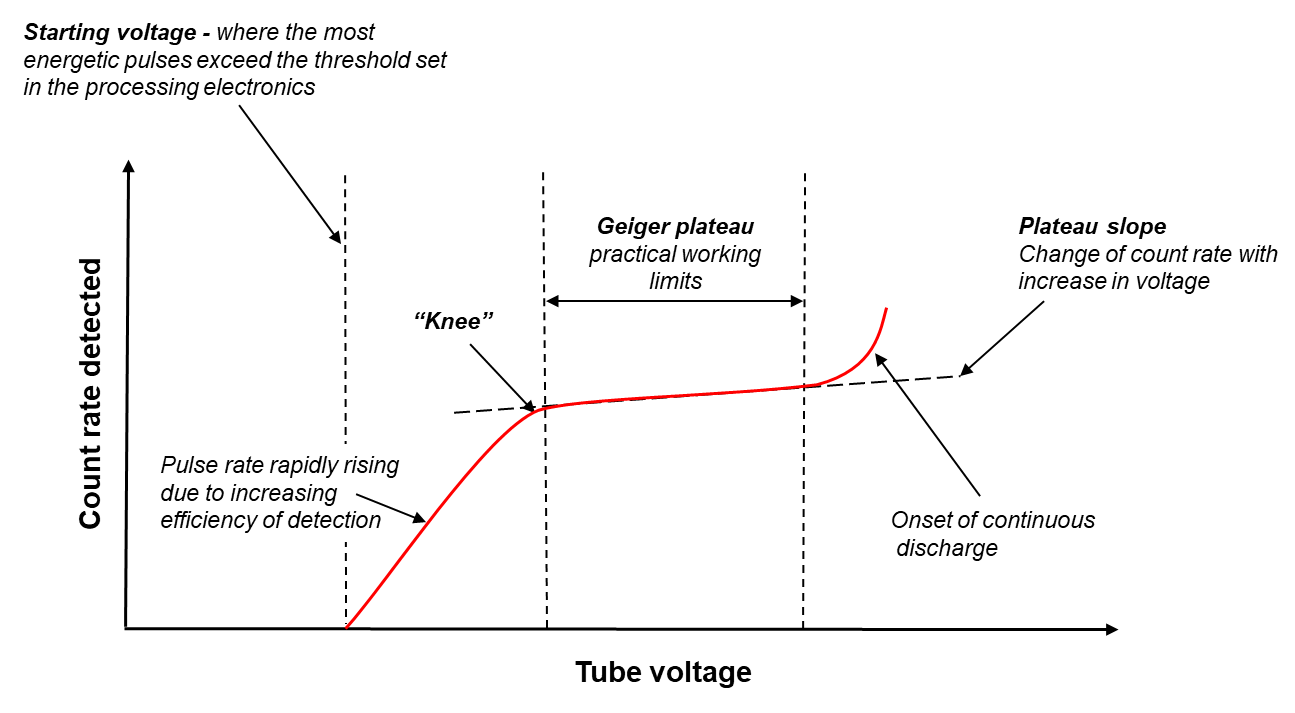
\includegraphics[scale = 0.38]{Figures/Geiger_plateau_curve.png}
        \caption{The characteristic curve of Geiger Muller tube response with constant radiation against varying tube voltage.}
        \label{fig:disc-1}
    \end{figure}
    \item The background counts correspond to  the counting rate measured in the absence of the radiation source. It is due to cosmic rays and any active sources in the experimental room.
    \item Dead time is the time interval, after the initiation of a discharge resulting in a normal pulse, during which the G.M. Tube is insensitive to further ionizing events.
    \begin{figure}
        \centering
        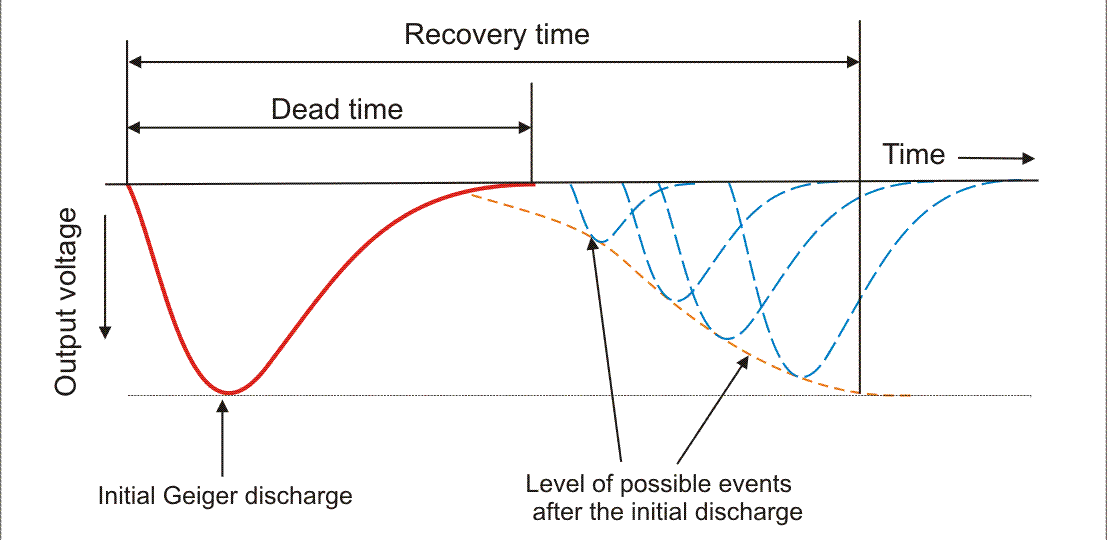
\includegraphics[scale = 0.29]{Figures/Dead_time_of_geiger_muller_tube.png}
        \caption{Dead time and recovery time in a Geiger Muller tube. The tube can produce no further pulses during the dead time, and only produces pulses of lesser height until the recovery time has elapsed.}
        \label{fig:disc-0}
    \end{figure}
    \item Resolution time is the minimum time interval between two distinct ionizing events which enables both to be counted independently or separately.
    \item Recovery time is the minimum time interval between the initiation of a normal size pulse and the initiation of the next pulse of normal size.
    \item The figure (\ref{fig:gaseous regions}) shows the relationship of the gaseous detection regions, using an experimental concept of applying a varying voltage to a cylindrical chamber which is subjected to ionising radiation. Alpha and beta particles are plotted to demonstrate the effect of different ionising energies, but the same principle extends to all forms of ionising radiation.
    \begin{figure}
        \centering
        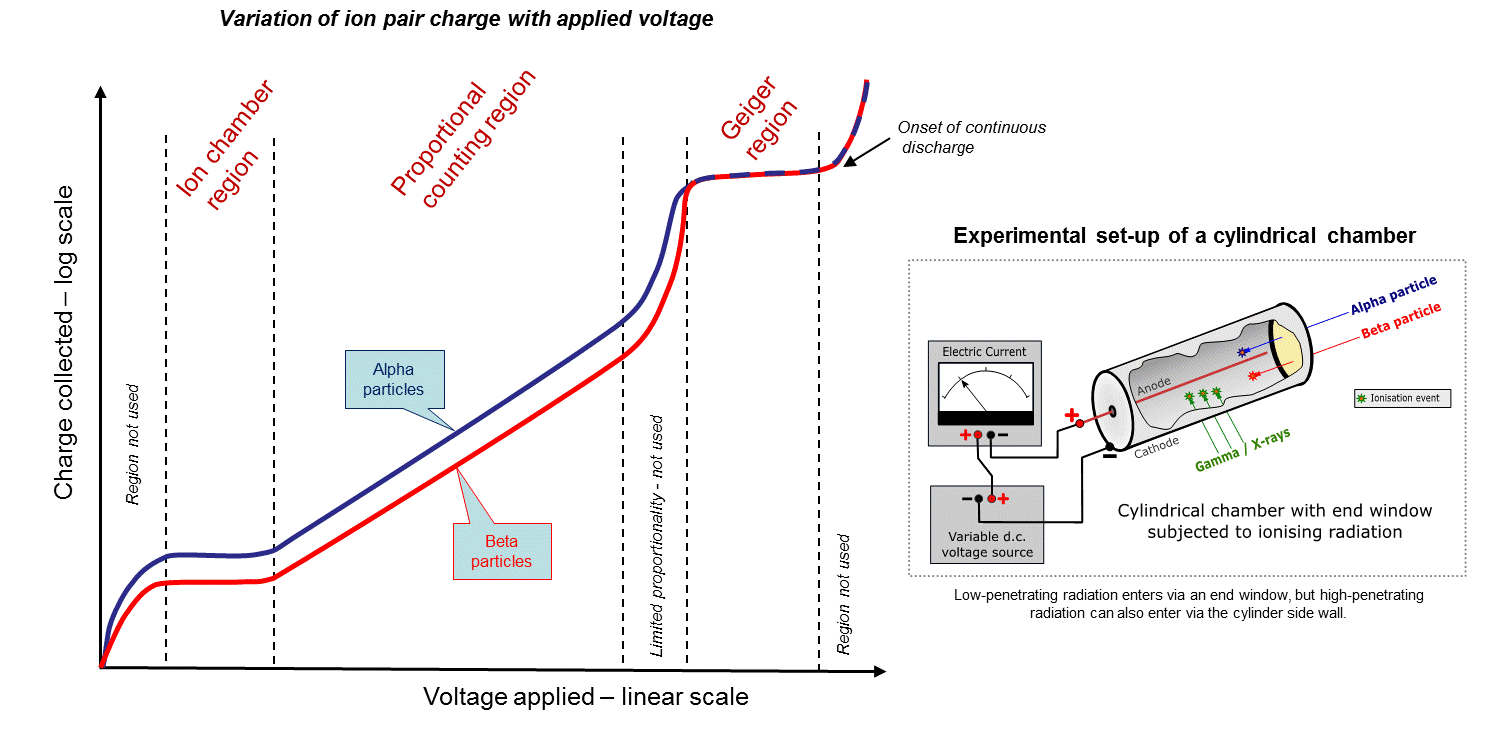
\includegraphics[scale = 0.20]{Figures/Detector_regions.png}
        \caption{Practical Gaseous Ionisation detection regions}
        \label{fig:gaseous regions}
    \end{figure}
    \item Normally the tube should be operated with an anode resistor of the value indicated in the measuring circuit, or higher. Decreasing the value of the anode resistor not only decreases the dead time but also the plateau length. A decrease in resistance below the limiting value may affect tube life and lead to its early destruction.
    \begin{figure}
        \centering
        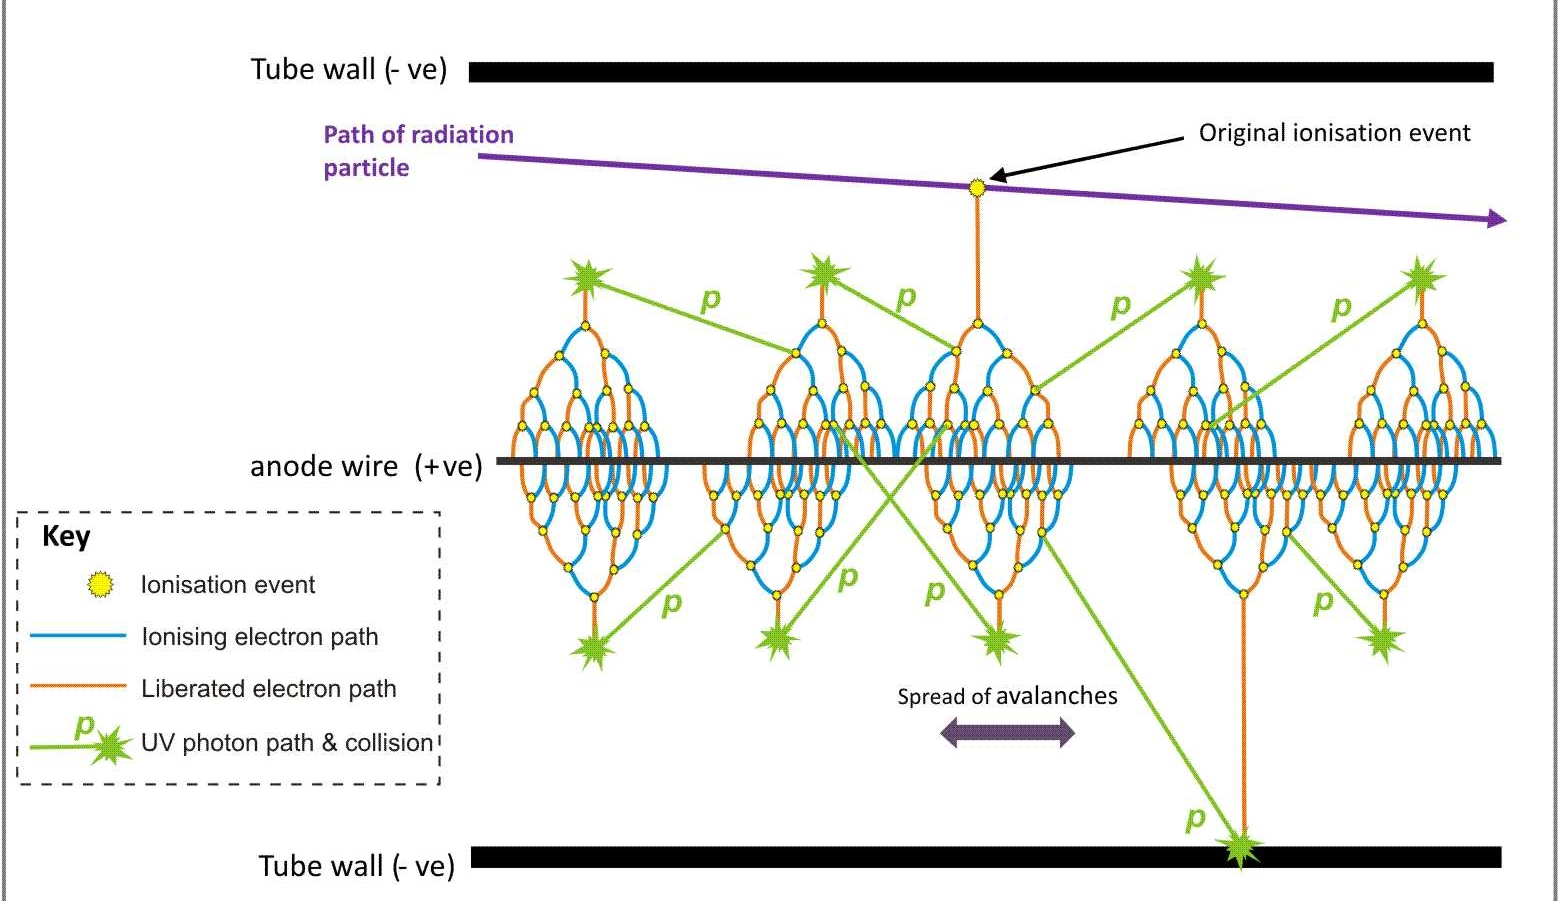
\includegraphics[scale = 0.3]{Figures/Spread_of_avalanches_in_G-M_tube.jpg}
        \caption{Visualization of the spread of Townsend avalanches by means of UV photons. This mechanism allows a single ionizing event to ionize all the gas surrounding the anode by triggering multiple avalanches.}
        \label{fig:disc-2}
    \end{figure}
    \item Avalanche effect in gas subject to ionising radiation between two plate electrodes. The original ionisation event liberates one electron, and each subsequent collision liberates a further electron, so two electrons emerge from each collision to sustain the avalanche.
    \begin{figure}
        \centering
        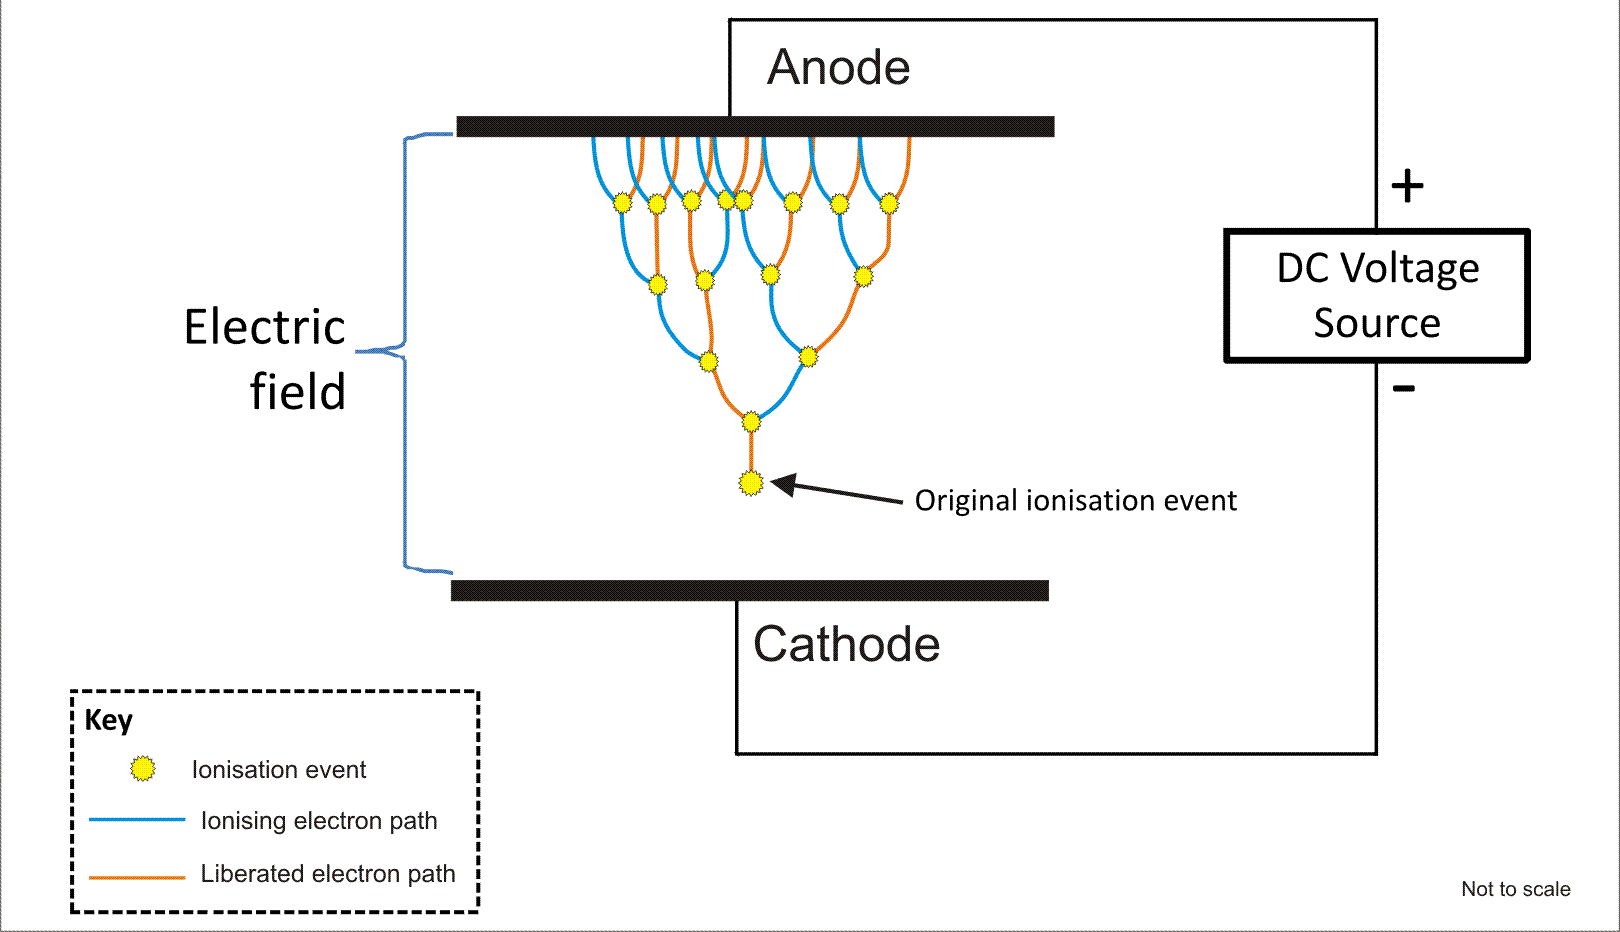
\includegraphics[scale = 0.2]{Figures/Electron_avalanche.png}
        \caption{Visualisation of Townsend avalanche}
        \label{fig:disc-3}
    \end{figure}
    \item The anode resistor should be connected directly to the anode connector of the tube to ensure that parasitic capacitances of leads will not excessively increase the capacitive load on the tube. An increase in capacitive load may increase the pulse amplitude, the pulse duration, the dead time and plateau slope. In addition the plateau will be shortened appreciably.
    \begin{figure}
        \centering
        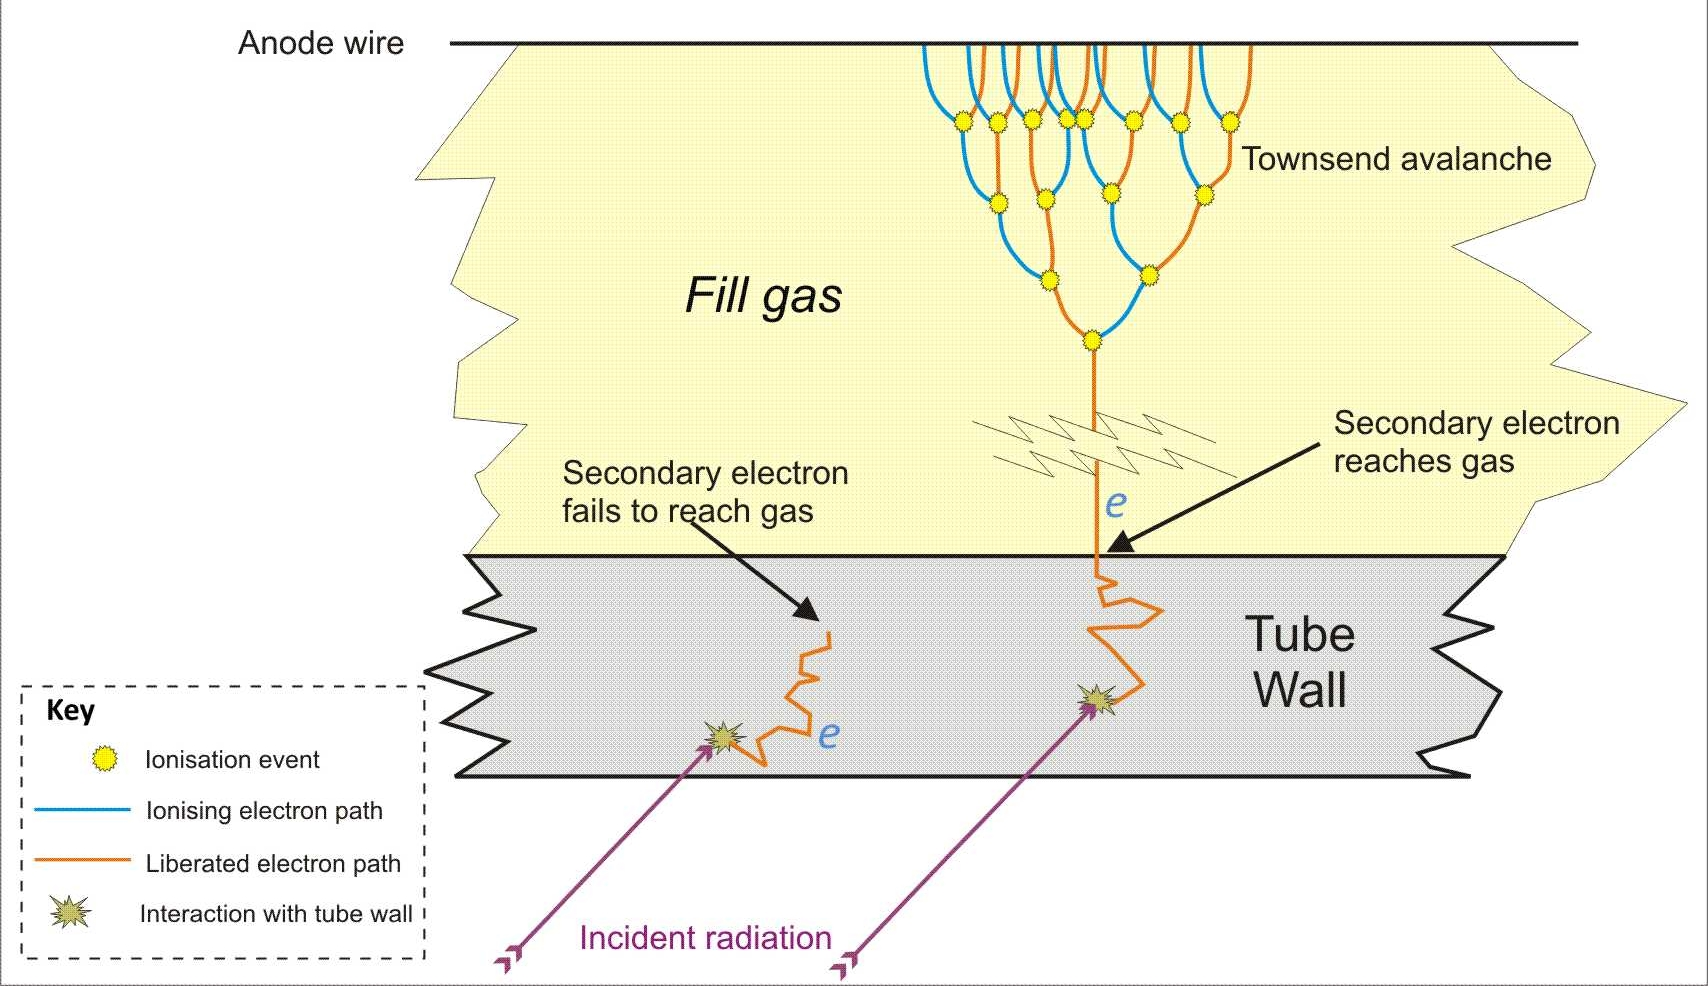
\includegraphics[scale = 0.29]{Figures/Geiger_gamma_interaction.jpg}
        \caption{Detection of gamma in a G-M tube with a thick-walled stainless steel cathode. Secondary electrons generated in the wall can reach the fill gas to produce avalanches.}
        \label{fig:disc-4}
    \end{figure}
    \item For continuous stable operation, it is recommended that the counting rate is adjusted to a value in the linear part of the counting rate/dose rate curve.
    \item At dose rates exceeding the recommended maximum, a G.M.Tube will produce the maximum number of counting pulses per second, limited by its dead time and the circuit in which it is incorporated. However, due to the characteristics of a specific circuit, the indicated counting rate may fall appreciably, even to zero. If dose rates exceeding 10 times the recommended maximum for window tubes, or 100 times for cylinder tubes, are likely to be encountered, it is advisable to use a circuit that continuously indicates saturation.
    \item The most important sources of background count are: Gamma radiation from the environment and from cosmic radiation, mesons from cosmic radiation, beta particles from contamination and impurities of the materials from which the detector itself is made, spontaneous discharge or pulses in the detector and the counting circuit that do not originate from radiation (Electronic noise).
    \item The operational life of a G.M. Tube is expressed in counts (discharge). Theoretically the quenching gas, ionized during a discharge, should be re-combined between discharges. However, minute quantities will be chemically bound, no longer taking part in the quenching process. This will lead to a gradual reduction of the plateau length and for a given working voltage to an increased counting rate. This will culminate in a continuous state of discharge of the tube rendering it useless.
    \item While handling the radioactive sources, utmost precautions should be taken.
\end{enumerate}


\end{document}
%
% ****** End of file apssamp.tex ******
